\documentclass[oneside]{book}
\usepackage[bookmarks=true, colorlinks, linkcolor=gray]{hyperref}
\usepackage[top=1in, bottom=1in, left=1.25in, right=1.25in]{geometry}
\usepackage{cite}
\usepackage{graphicx}
\usepackage{listings}
\usepackage{color}

% Packages required by doxygen
\usepackage{fixltx2e}
\usepackage{calc}
\usepackage{doxygen}
\usepackage[export]{adjustbox} % also loads graphicx
\usepackage{graphicx}
\usepackage[utf8]{inputenc}
\usepackage{makeidx}
\usepackage{multicol}
\usepackage{multirow}
\PassOptionsToPackage{warn}{textcomp}
\usepackage{textcomp}
\usepackage[nointegrals]{wasysym}
\usepackage[table]{xcolor}


% \renewcommand\thesection{\arabic{section}}

\definecolor{mygreen}{rgb}{0,0.6,0}
\definecolor{mygray}{rgb}{0.5,0.5,0.5}
\definecolor{mymauve}{rgb}{0.58,0,0.82}

\lstset{ %
  backgroundcolor=\color{white},   % choose the background color; you must add \usepackage{color} or \usepackage{xcolor}
  basicstyle=\footnotesize\ttfamily,        % the size of the fonts that are used for the code
  breakatwhitespace=false,         % sets if automatic breaks should only happen at whitespace
  breaklines=true,                 % sets automatic line breaking
  captionpos=b,                    % sets the caption-position to bottom
  commentstyle=\color{mygreen}\ttfamily,    % comment style
  frame=single,	                   % adds a frame around the code
  keepspaces=true,                 % keeps spaces in text, useful for keeping indentation of code (possibly needs columns=flexible)
  keywordstyle=\color{blue},       % keyword style
  language=C++,                    % the language of the code
  rulecolor=\color{black},         % if not set, the frame-color may be changed on line-breaks within not-black text (e.g. comments (green here))
  showspaces=false,                % show spaces everywhere adding particular underscores; it overrides 'showstringspaces'
  showstringspaces=false,          % underline spaces within strings only
  showtabs=false,                  % show tabs within strings adding particular underscores
  stepnumber=2,                    % the step between two line-numbers. If it's 1, each line will be numbered
  stringstyle=\color{mymauve},     % string literal style
  tabsize=2,	                   % sets default tabsize to 2 spaces
}

\usepackage{caption}
\captionsetup{labelsep=space,justification=centering,font={bf},singlelinecheck=off,skip=4pt,position=top}

% Add search path
\makeatletter
\providecommand*\input@path{}
\newcommand*\addinputpath[1]{%
  \expandafter\def\expandafter\input@path
  \expandafter{\input@path#1}}%
\addinputpath{{doxygen/}}
\makeatother

\graphicspath{{doxygen/}{UML/}}

% �½ڲ���ҳ
\usepackage{xpatch}
\makeatletter
\xpatchcmd{\chapter}
  {\if@openright\cleardoublepage\else\clearpage\fi}{\par\relax}
  {}{}
\makeatother

\title{Individual Project 2\\ Constructing Minimum Spanning Trees\\ Software Design Document}
\author{Zhang Huimeng, 2015011280}

\begin{document}

\maketitle
\author
\clearpage

\tableofcontents
\clearpage


\part{Introduction}

    \chapter{Purpose}

        This software design document describes the architecture and system design of project ComputeMST. This is a homework of Fundamentals of Object-Oriented Programming class, Spring 2016. The homework requirement is as follows:

         (II) Project: On Constructing Minimum Spanning Trees (Difficulty: 1.1)

        Requirements and TIPS:

        (1) Implement the MST algorithm based on Voronoi diagram for computing Euclidean minimum spanning trees in 2D plane.

        (2) Please refer to \href{http://www.cs.princeton.edu/courses/archive/spr07/cos226/lectures/mst.pdf}{the following link} for MST construction algorithms. Either Prim's or Kruskal's algorithm is ok. Please refer to Page 39 for the idea of using Voronoi for MST computation.

        (3) Use the \href{http://www.cgal.org/}{CGAL Library} for constructing the Voronoi diagram and Delaunay triangulation.

        (4) Randomly generate 5 different testcases with more than 5000 points without duplicates to test the implemented method.

        (5) It is suggested that a validity checking function be implemented to verify the experimental results are correct. For example, you may directly apply Prim's or Kruskal's MST algorithm on the testcase to verify that the MST trees are correct.

        (6) Report the statistics of the experimental results, e.g., total runtime, total number of points, total length of the MST edges, etc. Figures and tables on the experimental results are welcome.

        (7) [This is not mandatory to finish, but it is a challenging topic] Again, can you compute the top K ($1 <= K <= 20$) minimum spanning trees?
    
    \chapter{Scope}

        I implemented the first six requirements of the homework, mainly using CGAL and Kruskal's MST algorithm. The program can load input from file or randomly generate input for itself; it has a GUI interface and can print results of the MST computation to file.

    \chapter{Definitions and Acronyms}
        
        


\part{System Overview}
    
    The program can compute Delaunay triangulation (via CGAL library) and MST for up to 10000 points in a 2-dimensional plane in 1 or 2 seconds. It can output the result to file. Also, it has a interface written with Freeglut.
    
\clearpage


\part{System Architecture}

    \chapter{Architectural Design} % ������ϵͳ����Ϊ����ģ�飬����ÿ��ģ��֮��Ĺ��ܺ��໥��ϵ

        The program can be divided into three parts: the Basics part, the Computational part and the Display part. 
        
        \begin{center}
        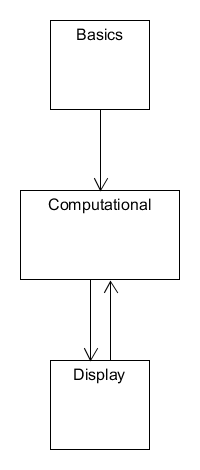
\includegraphics[width=\linewidth / 2]{main.png}
        \end{center}
        
        The basics part provides some useful tools for the Computational part, like statistics and timer.
        
        The computational part does the computation, and interacts with the Display part to provide a workable interface.
        
        The display part deals with the interface and user input.

    \chapter{Decomposition Description}
    
        \section{Basics}
        
            The \hyperlink{classcmst_1_1_stat}{Stat} class deals with statistics. It receives data in the form of floating-point number and can work continuously. It calculates the mean, maximum, minimum and standard deviation of the data.
        
            \begin{center}
            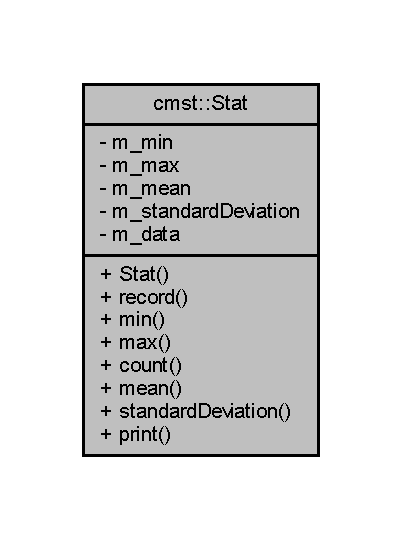
\includegraphics[width=\linewidth / 2]{classcmst_1_1_stat__coll__graph}
            \end{center}
            
            
        
        \section{Computational}
            
            The \hyperlink{classcmst_1_1_point2_d}{Point2D}, \hyperlink{classcmst_1_1_edge2_d}{Edge2D} and \hyperlink{classcmst_1_1_index_edge2_d}{IndexEdge2D} classes are the basic 2-dimensional computational geometry classes.

            \begin{center}
            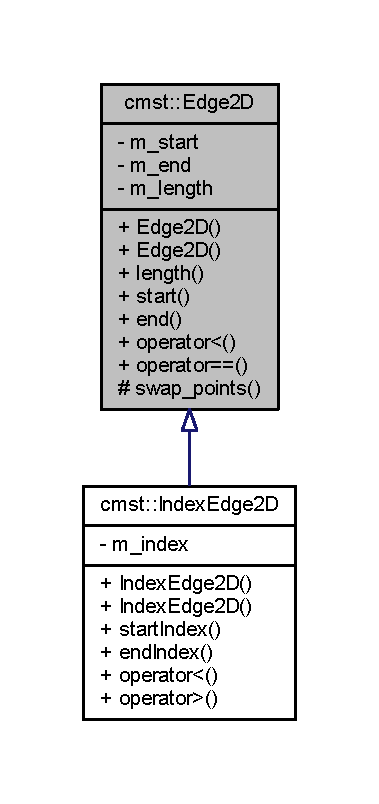
\includegraphics[width=\linewidth / 2]{classcmst_1_1_edge2_d__inherit__graph}
            \end{center}

            \begin{center}
            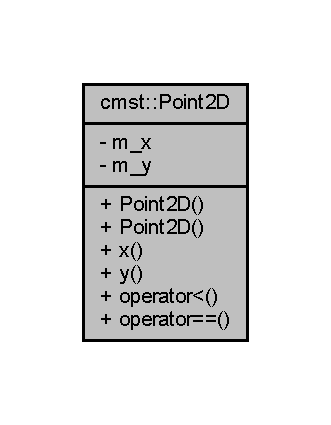
\includegraphics[width=\linewidth / 2]{classcmst_1_1_point2_d__coll__graph}
            \end{center}
        
        \section{Display}

    \chapter{Design Rationale}

\clearpage


\part{Data Design}

    \chapter{Data Description} % data structure, data storage, process and organization

    \chapter{Data Dictionary} % list the objects and its attributes, methods and method parameters

\clearpage


\part{Human Interface Design}

    \chapter{Overview of Human Interface}

    \chapter{Screen Images}

    \chapter{Screen Objects and Actions}

\clearpage


\part{Design Patterns}

\clearpage


\part{Component Design}
%--- Begin generated contents ---
\chapter{Namespace Index}
\section{Namespace List}
Here is a list of all namespaces with brief descriptions\+:\begin{DoxyCompactList}
\item\contentsline{section}{\hyperlink{namespacecmst}{cmst} }{\pageref{namespacecmst}}{}
\end{DoxyCompactList}

\chapter{Hierarchical Index}
\section{Class Hierarchy}
This inheritance list is sorted roughly, but not completely, alphabetically:\begin{DoxyCompactList}
\item \contentsline{section}{Delaunay}{\pageref{class_delaunay}}{}
\item \contentsline{section}{Edge}{\pageref{class_edge}}{}
\item \contentsline{section}{cmst::Edge2D}{\pageref{classcmst_1_1_edge2_d}}{}
\begin{DoxyCompactList}
\item \contentsline{section}{cmst::IndexEdge2D}{\pageref{classcmst_1_1_index_edge2_d}}{}
\end{DoxyCompactList}
\item \contentsline{section}{cmst::Graph2D}{\pageref{classcmst_1_1_graph2_d}}{}
\item \contentsline{section}{cmst::Point2D}{\pageref{classcmst_1_1_point2_d}}{}
\item \contentsline{section}{cmst::Stat}{\pageref{classcmst_1_1_stat}}{}
\item \contentsline{section}{cmst::Window::Test}{\pageref{structcmst_1_1_window_1_1_test}}{}
\item \contentsline{section}{cmst::Timer}{\pageref{classcmst_1_1_timer}}{}
\item \contentsline{section}{Triangle}{\pageref{class_triangle}}{}
\item \contentsline{section}{Vec2f}{\pageref{class_vec2f}}{}
\item \contentsline{section}{cmst::Window}{\pageref{classcmst_1_1_window}}{}
\end{DoxyCompactList}

\chapter{Class Index}
\section{Class List}
Here are the classes, structs, unions and interfaces with brief descriptions\+:\begin{DoxyCompactList}
\item\contentsline{section}{\hyperlink{classcmst_1_1_edge2_d}{cmst\+::\+Edge2D} }{\pageref{classcmst_1_1_edge2_d}}{}
\item\contentsline{section}{\hyperlink{classcmst_1_1_graph2_d}{cmst\+::\+Graph2D} }{\pageref{classcmst_1_1_graph2_d}}{}
\item\contentsline{section}{\hyperlink{classcmst_1_1_index_edge2_d}{cmst\+::\+Index\+Edge2D} \\*Edge with start and end point indices in an array }{\pageref{classcmst_1_1_index_edge2_d}}{}
\item\contentsline{section}{\hyperlink{classcmst_1_1_point2_d}{cmst\+::\+Point2D} \\*Points in a 2D plane }{\pageref{classcmst_1_1_point2_d}}{}
\item\contentsline{section}{\hyperlink{structcmst_1_1_graph2_d_1_1_s_t}{cmst\+::\+Graph2\+D\+::\+ST} \\*Store a spanning tree of the graph }{\pageref{structcmst_1_1_graph2_d_1_1_s_t}}{}
\item\contentsline{section}{\hyperlink{classcmst_1_1_stat}{cmst\+::\+Stat} }{\pageref{classcmst_1_1_stat}}{}
\item\contentsline{section}{\hyperlink{structcmst_1_1_window_1_1_test}{cmst\+::\+Window\+::\+Test} }{\pageref{structcmst_1_1_window_1_1_test}}{}
\item\contentsline{section}{\hyperlink{classcmst_1_1_timer}{cmst\+::\+Timer} }{\pageref{classcmst_1_1_timer}}{}
\item\contentsline{section}{\hyperlink{classcmst_1_1_window}{cmst\+::\+Window} }{\pageref{classcmst_1_1_window}}{}
\end{DoxyCompactList}

\chapter{Namespace Documentation}
\hypertarget{namespacecmst}{}\section{cmst Namespace Reference}
\label{namespacecmst}\index{cmst@{cmst}}
\subsection*{Classes}
\begin{DoxyCompactItemize}
\item 
class \hyperlink{classcmst_1_1_edge2_d}{Edge2D}
\item 
class \hyperlink{classcmst_1_1_graph2_d}{Graph2D}
\item 
class \hyperlink{classcmst_1_1_index_edge2_d}{Index\+Edge2D}
\item 
class \hyperlink{classcmst_1_1_point2_d}{Point2D}
\item 
class \hyperlink{classcmst_1_1_stat}{Stat}
\item 
class \hyperlink{classcmst_1_1_timer}{Timer}
\item 
class \hyperlink{classcmst_1_1_window}{Window}
\end{DoxyCompactItemize}
\subsection*{Enumerations}
\begin{DoxyCompactItemize}
\item 
enum \hyperlink{namespacecmst_a8dff7ccfde8a2770160b5f8dbf81c3b9}{Menu} \{ \\*
\hyperlink{namespacecmst_a8dff7ccfde8a2770160b5f8dbf81c3b9acc1b341b1550c4009942f0a14b433fb5}{N\+EW}, 
\hyperlink{namespacecmst_a8dff7ccfde8a2770160b5f8dbf81c3b9a5c1bbae108fea09abee0ae385bc729bf}{N\+E\+W\+\_\+4\+\_\+10}, 
\hyperlink{namespacecmst_a8dff7ccfde8a2770160b5f8dbf81c3b9a613b1d9e468c6e26e23c33a2abb2833e}{N\+E\+W\+\_\+11\+\_\+100}, 
\hyperlink{namespacecmst_a8dff7ccfde8a2770160b5f8dbf81c3b9a7ca958e9941ebe27acf2ae7511b735ba}{N\+E\+W\+\_\+101\+\_\+1000}, 
\\*
\hyperlink{namespacecmst_a8dff7ccfde8a2770160b5f8dbf81c3b9a35fe2b5c1c0015c3aee5049bee8b8acd}{N\+E\+W\+\_\+1001\+\_\+5000}, 
\hyperlink{namespacecmst_a8dff7ccfde8a2770160b5f8dbf81c3b9a73f732474a8fd1746e18e85ac18965f0}{N\+E\+W\+\_\+5001\+\_\+10000}, 
\hyperlink{namespacecmst_a8dff7ccfde8a2770160b5f8dbf81c3b9a4484f6b658f88772d77bfeaaa19b7a11}{S\+H\+OW}, 
\hyperlink{namespacecmst_a8dff7ccfde8a2770160b5f8dbf81c3b9acb33c06abf6f54d270a6a6f26b3b0ec4}{S\+H\+O\+W\+\_\+\+V\+O\+R\+O\+N\+OI}, 
\\*
\hyperlink{namespacecmst_a8dff7ccfde8a2770160b5f8dbf81c3b9a4a94d06c45900d709f4714d9fdebb3f0}{S\+H\+O\+W\+\_\+\+D\+E\+L\+A\+U\+N\+AY}, 
\hyperlink{namespacecmst_a8dff7ccfde8a2770160b5f8dbf81c3b9a95c752e50b27aaae9aa758293828007f}{T\+E\+ST}, 
\hyperlink{namespacecmst_a8dff7ccfde8a2770160b5f8dbf81c3b9a9996ad31ad035f42371059ad53098246}{T\+E\+S\+T\+\_\+5}, 
\hyperlink{namespacecmst_a8dff7ccfde8a2770160b5f8dbf81c3b9a3f5dd18e08446227f6ce81fed096c339}{T\+E\+S\+T\+\_\+20}, 
\\*
\hyperlink{namespacecmst_a8dff7ccfde8a2770160b5f8dbf81c3b9af46a16cac81f794824d0d87fb5588e33}{Q\+U\+IT}
 \}\begin{DoxyCompactList}\small\item\em Return values for G\+L\+UT menus. \end{DoxyCompactList}
\end{DoxyCompactItemize}
\subsection*{Functions}
\begin{DoxyCompactItemize}
\item 
int \hyperlink{namespacecmst_a844037f018f3d5b7b1f1a5f4463da501}{random\+Int} (int a, int b)
\item 
double \hyperlink{namespacecmst_a8df08a5847caeb65a6606968e40f336f}{random\+Double} (double a, double b)
\item 
std\+::vector$<$ \hyperlink{classcmst_1_1_point2_d}{Point2D} $>$ \hyperlink{namespacecmst_abd1822f67dc5d2be959508e628be0633}{Testcase\+Generator} (int num\+\_\+lower\+\_\+bound=100, int num\+\_\+upper\+\_\+bound=500, double x\+\_\+upper\+\_\+bound=M\+A\+X\+\_\+X, double y\+\_\+upper\+\_\+bound=M\+A\+X\+\_\+Y)
\end{DoxyCompactItemize}


\subsection{Enumeration Type Documentation}
\index{cmst@{cmst}!Menu@{Menu}}
\index{Menu@{Menu}!cmst@{cmst}}
\subsubsection[{\texorpdfstring{Menu}{Menu}}]{\setlength{\rightskip}{0pt plus 5cm}enum {\bf cmst\+::\+Menu}}\hypertarget{namespacecmst_a8dff7ccfde8a2770160b5f8dbf81c3b9}{}\label{namespacecmst_a8dff7ccfde8a2770160b5f8dbf81c3b9}


Return values for G\+L\+UT menus. 

\begin{Desc}
\item[Enumerator]\par
\begin{description}
\index{N\+EW@{N\+EW}!cmst@{cmst}}\index{cmst@{cmst}!N\+EW@{N\+EW}}\item[{\em 
N\+EW\hypertarget{namespacecmst_a8dff7ccfde8a2770160b5f8dbf81c3b9acc1b341b1550c4009942f0a14b433fb5}{}\label{namespacecmst_a8dff7ccfde8a2770160b5f8dbf81c3b9acc1b341b1550c4009942f0a14b433fb5}
}]\index{N\+E\+W\+\_\+4\+\_\+10@{N\+E\+W\+\_\+4\+\_\+10}!cmst@{cmst}}\index{cmst@{cmst}!N\+E\+W\+\_\+4\+\_\+10@{N\+E\+W\+\_\+4\+\_\+10}}\item[{\em 
N\+E\+W\+\_\+4\+\_\+10\hypertarget{namespacecmst_a8dff7ccfde8a2770160b5f8dbf81c3b9a5c1bbae108fea09abee0ae385bc729bf}{}\label{namespacecmst_a8dff7ccfde8a2770160b5f8dbf81c3b9a5c1bbae108fea09abee0ae385bc729bf}
}]\index{N\+E\+W\+\_\+11\+\_\+100@{N\+E\+W\+\_\+11\+\_\+100}!cmst@{cmst}}\index{cmst@{cmst}!N\+E\+W\+\_\+11\+\_\+100@{N\+E\+W\+\_\+11\+\_\+100}}\item[{\em 
N\+E\+W\+\_\+11\+\_\+100\hypertarget{namespacecmst_a8dff7ccfde8a2770160b5f8dbf81c3b9a613b1d9e468c6e26e23c33a2abb2833e}{}\label{namespacecmst_a8dff7ccfde8a2770160b5f8dbf81c3b9a613b1d9e468c6e26e23c33a2abb2833e}
}]\index{N\+E\+W\+\_\+101\+\_\+1000@{N\+E\+W\+\_\+101\+\_\+1000}!cmst@{cmst}}\index{cmst@{cmst}!N\+E\+W\+\_\+101\+\_\+1000@{N\+E\+W\+\_\+101\+\_\+1000}}\item[{\em 
N\+E\+W\+\_\+101\+\_\+1000\hypertarget{namespacecmst_a8dff7ccfde8a2770160b5f8dbf81c3b9a7ca958e9941ebe27acf2ae7511b735ba}{}\label{namespacecmst_a8dff7ccfde8a2770160b5f8dbf81c3b9a7ca958e9941ebe27acf2ae7511b735ba}
}]\index{N\+E\+W\+\_\+1001\+\_\+5000@{N\+E\+W\+\_\+1001\+\_\+5000}!cmst@{cmst}}\index{cmst@{cmst}!N\+E\+W\+\_\+1001\+\_\+5000@{N\+E\+W\+\_\+1001\+\_\+5000}}\item[{\em 
N\+E\+W\+\_\+1001\+\_\+5000\hypertarget{namespacecmst_a8dff7ccfde8a2770160b5f8dbf81c3b9a35fe2b5c1c0015c3aee5049bee8b8acd}{}\label{namespacecmst_a8dff7ccfde8a2770160b5f8dbf81c3b9a35fe2b5c1c0015c3aee5049bee8b8acd}
}]\index{N\+E\+W\+\_\+5001\+\_\+10000@{N\+E\+W\+\_\+5001\+\_\+10000}!cmst@{cmst}}\index{cmst@{cmst}!N\+E\+W\+\_\+5001\+\_\+10000@{N\+E\+W\+\_\+5001\+\_\+10000}}\item[{\em 
N\+E\+W\+\_\+5001\+\_\+10000\hypertarget{namespacecmst_a8dff7ccfde8a2770160b5f8dbf81c3b9a73f732474a8fd1746e18e85ac18965f0}{}\label{namespacecmst_a8dff7ccfde8a2770160b5f8dbf81c3b9a73f732474a8fd1746e18e85ac18965f0}
}]\index{S\+H\+OW@{S\+H\+OW}!cmst@{cmst}}\index{cmst@{cmst}!S\+H\+OW@{S\+H\+OW}}\item[{\em 
S\+H\+OW\hypertarget{namespacecmst_a8dff7ccfde8a2770160b5f8dbf81c3b9a4484f6b658f88772d77bfeaaa19b7a11}{}\label{namespacecmst_a8dff7ccfde8a2770160b5f8dbf81c3b9a4484f6b658f88772d77bfeaaa19b7a11}
}]\index{S\+H\+O\+W\+\_\+\+V\+O\+R\+O\+N\+OI@{S\+H\+O\+W\+\_\+\+V\+O\+R\+O\+N\+OI}!cmst@{cmst}}\index{cmst@{cmst}!S\+H\+O\+W\+\_\+\+V\+O\+R\+O\+N\+OI@{S\+H\+O\+W\+\_\+\+V\+O\+R\+O\+N\+OI}}\item[{\em 
S\+H\+O\+W\+\_\+\+V\+O\+R\+O\+N\+OI\hypertarget{namespacecmst_a8dff7ccfde8a2770160b5f8dbf81c3b9acb33c06abf6f54d270a6a6f26b3b0ec4}{}\label{namespacecmst_a8dff7ccfde8a2770160b5f8dbf81c3b9acb33c06abf6f54d270a6a6f26b3b0ec4}
}]\index{S\+H\+O\+W\+\_\+\+D\+E\+L\+A\+U\+N\+AY@{S\+H\+O\+W\+\_\+\+D\+E\+L\+A\+U\+N\+AY}!cmst@{cmst}}\index{cmst@{cmst}!S\+H\+O\+W\+\_\+\+D\+E\+L\+A\+U\+N\+AY@{S\+H\+O\+W\+\_\+\+D\+E\+L\+A\+U\+N\+AY}}\item[{\em 
S\+H\+O\+W\+\_\+\+D\+E\+L\+A\+U\+N\+AY\hypertarget{namespacecmst_a8dff7ccfde8a2770160b5f8dbf81c3b9a4a94d06c45900d709f4714d9fdebb3f0}{}\label{namespacecmst_a8dff7ccfde8a2770160b5f8dbf81c3b9a4a94d06c45900d709f4714d9fdebb3f0}
}]\index{T\+E\+ST@{T\+E\+ST}!cmst@{cmst}}\index{cmst@{cmst}!T\+E\+ST@{T\+E\+ST}}\item[{\em 
T\+E\+ST\hypertarget{namespacecmst_a8dff7ccfde8a2770160b5f8dbf81c3b9a95c752e50b27aaae9aa758293828007f}{}\label{namespacecmst_a8dff7ccfde8a2770160b5f8dbf81c3b9a95c752e50b27aaae9aa758293828007f}
}]\index{T\+E\+S\+T\+\_\+5@{T\+E\+S\+T\+\_\+5}!cmst@{cmst}}\index{cmst@{cmst}!T\+E\+S\+T\+\_\+5@{T\+E\+S\+T\+\_\+5}}\item[{\em 
T\+E\+S\+T\+\_\+5\hypertarget{namespacecmst_a8dff7ccfde8a2770160b5f8dbf81c3b9a9996ad31ad035f42371059ad53098246}{}\label{namespacecmst_a8dff7ccfde8a2770160b5f8dbf81c3b9a9996ad31ad035f42371059ad53098246}
}]\index{T\+E\+S\+T\+\_\+20@{T\+E\+S\+T\+\_\+20}!cmst@{cmst}}\index{cmst@{cmst}!T\+E\+S\+T\+\_\+20@{T\+E\+S\+T\+\_\+20}}\item[{\em 
T\+E\+S\+T\+\_\+20\hypertarget{namespacecmst_a8dff7ccfde8a2770160b5f8dbf81c3b9a3f5dd18e08446227f6ce81fed096c339}{}\label{namespacecmst_a8dff7ccfde8a2770160b5f8dbf81c3b9a3f5dd18e08446227f6ce81fed096c339}
}]\index{Q\+U\+IT@{Q\+U\+IT}!cmst@{cmst}}\index{cmst@{cmst}!Q\+U\+IT@{Q\+U\+IT}}\item[{\em 
Q\+U\+IT\hypertarget{namespacecmst_a8dff7ccfde8a2770160b5f8dbf81c3b9af46a16cac81f794824d0d87fb5588e33}{}\label{namespacecmst_a8dff7ccfde8a2770160b5f8dbf81c3b9af46a16cac81f794824d0d87fb5588e33}
}]\end{description}
\end{Desc}


\subsection{Function Documentation}
\index{cmst@{cmst}!random\+Double@{random\+Double}}
\index{random\+Double@{random\+Double}!cmst@{cmst}}
\subsubsection[{\texorpdfstring{random\+Double(double a, double b)}{randomDouble(double a, double b)}}]{\setlength{\rightskip}{0pt plus 5cm}double cmst\+::random\+Double (
\begin{DoxyParamCaption}
\item[{double}]{a, }
\item[{double}]{b}
\end{DoxyParamCaption}
)}\hypertarget{namespacecmst_a8df08a5847caeb65a6606968e40f336f}{}\label{namespacecmst_a8df08a5847caeb65a6606968e40f336f}
Generate a floating-\/point number in the range \mbox{[}a, b\mbox{]}

Needs to be improved using other random classes 

Here is the caller graph for this function\+:
% FIG 0


\index{cmst@{cmst}!random\+Int@{random\+Int}}
\index{random\+Int@{random\+Int}!cmst@{cmst}}
\subsubsection[{\texorpdfstring{random\+Int(int a, int b)}{randomInt(int a, int b)}}]{\setlength{\rightskip}{0pt plus 5cm}int cmst\+::random\+Int (
\begin{DoxyParamCaption}
\item[{int}]{a, }
\item[{int}]{b}
\end{DoxyParamCaption}
)}\hypertarget{namespacecmst_a844037f018f3d5b7b1f1a5f4463da501}{}\label{namespacecmst_a844037f018f3d5b7b1f1a5f4463da501}
Generate an integer in the range \mbox{[}a, b\mbox{]}

Needs to be improved using other random classes 

Here is the caller graph for this function\+:
% FIG 1


\index{cmst@{cmst}!Testcase\+Generator@{Testcase\+Generator}}
\index{Testcase\+Generator@{Testcase\+Generator}!cmst@{cmst}}
\subsubsection[{\texorpdfstring{Testcase\+Generator(int num\+\_\+lower\+\_\+bound=100, int num\+\_\+upper\+\_\+bound=500, double x\+\_\+upper\+\_\+bound=\+M\+A\+X\+\_\+\+X, double y\+\_\+upper\+\_\+bound=\+M\+A\+X\+\_\+\+Y)}{TestcaseGenerator(int num_lower_bound=100, int num_upper_bound=500, double x_upper_bound=MAX_X, double y_upper_bound=MAX_Y)}}]{\setlength{\rightskip}{0pt plus 5cm}std\+::vector$<$ {\bf cmst\+::\+Point2D} $>$ cmst\+::\+Testcase\+Generator (
\begin{DoxyParamCaption}
\item[{int}]{num\+\_\+lower\+\_\+bound = {\ttfamily 100}, }
\item[{int}]{num\+\_\+upper\+\_\+bound = {\ttfamily 500}, }
\item[{double}]{x\+\_\+upper\+\_\+bound = {\ttfamily MAX\+\_\+X}, }
\item[{double}]{y\+\_\+upper\+\_\+bound = {\ttfamily MAX\+\_\+Y}}
\end{DoxyParamCaption}
)}\hypertarget{namespacecmst_abd1822f67dc5d2be959508e628be0633}{}\label{namespacecmst_abd1822f67dc5d2be959508e628be0633}
To-\/do\+: output the testcase file to ../testcase; Add erase and unique 

Here is the call graph for this function\+:
% FIG 2




Here is the caller graph for this function\+:
% FIG 3



\chapter{Class Documentation}
\hypertarget{class_delaunay}{}\section{Delaunay Class Reference}
\label{class_delaunay}\index{Delaunay@{Delaunay}}


{\ttfamily \#include $<$delaunay.h$>$}



Collaboration diagram for Delaunay:
% FIG 0
\subsection*{Public Member Functions}
\begin{DoxyCompactItemize}
\item 
std::vector$<$ \hyperlink{class_triangle}{Triangle} $>$ \hyperlink{class_delaunay_a97f07ff9e702dd4592fe353805a9f82c}{triangulate} (std::vector$<$ \hyperlink{class_vec2f}{Vec2f} $>$ \&vertices)
\item 
std::vector$<$ \hyperlink{class_triangle}{Triangle} $>$ \hyperlink{class_delaunay_a15d2799c1fa1b237e4f0afad610517c2}{getTriangles} ()
\item 
std::vector$<$ \hyperlink{class_edge}{Edge} $>$ \hyperlink{class_delaunay_a8ca53e3d46f367fc879de1905d8bbf3b}{getEdges} ()
\end{DoxyCompactItemize}
\subsection*{Private Attributes}
\begin{DoxyCompactItemize}
\item 
std::vector$<$ \hyperlink{class_triangle}{Triangle} $>$ \hyperlink{class_delaunay_a7f57c36e1eed644efe9e469c5212a826}{\_triangles}
\item 
std::vector$<$ \hyperlink{class_edge}{Edge} $>$ \hyperlink{class_delaunay_a6e53063d9dd4df3936c14165e64e482f}{\_edges}
\end{DoxyCompactItemize}


\subsection{Member Function Documentation}
\index{Delaunay@{Delaunay}!getEdges@{getEdges}}
\index{getEdges@{getEdges}!Delaunay@{Delaunay}}
\subsubsection[{\texorpdfstring{getEdges()}{getEdges()}}]{\setlength{\rightskip}{0pt plus 5cm}std::vector$<${\bf Edge}$>$ Delaunay::getEdges (
\begin{DoxyParamCaption}
{}
\end{DoxyParamCaption}
)\hspace{0.3cm}{\ttfamily [inline]}}\hypertarget{class_delaunay_a8ca53e3d46f367fc879de1905d8bbf3b}{}\label{class_delaunay_a8ca53e3d46f367fc879de1905d8bbf3b}
\index{Delaunay@{Delaunay}!getTriangles@{getTriangles}}
\index{getTriangles@{getTriangles}!Delaunay@{Delaunay}}
\subsubsection[{\texorpdfstring{getTriangles()}{getTriangles()}}]{\setlength{\rightskip}{0pt plus 5cm}std::vector$<${\bf Triangle}$>$ Delaunay::getTriangles (
\begin{DoxyParamCaption}
{}
\end{DoxyParamCaption}
)\hspace{0.3cm}{\ttfamily [inline]}}\hypertarget{class_delaunay_a15d2799c1fa1b237e4f0afad610517c2}{}\label{class_delaunay_a15d2799c1fa1b237e4f0afad610517c2}
\index{Delaunay@{Delaunay}!triangulate@{triangulate}}
\index{triangulate@{triangulate}!Delaunay@{Delaunay}}
\subsubsection[{\texorpdfstring{triangulate(std::vector$<$ Vec2f $>$ \&vertices)}{triangulate(std::vector< Vec2f > &vertices)}}]{\setlength{\rightskip}{0pt plus 5cm}std::vector$<$ {\bf Triangle} $>$ Delaunay::triangulate (
\begin{DoxyParamCaption}
\item[{std::vector$<$ {\bf Vec2f} $>$ \&}]{vertices}
\end{DoxyParamCaption}
)}\hypertarget{class_delaunay_a97f07ff9e702dd4592fe353805a9f82c}{}\label{class_delaunay_a97f07ff9e702dd4592fe353805a9f82c}


Here is the call graph for this function:
% FIG 1




\subsection{Member Data Documentation}
\index{Delaunay@{Delaunay}!\_edges@{\_edges}}
\index{\_edges@{\_edges}!Delaunay@{Delaunay}}
\subsubsection[{\texorpdfstring{\_edges}{_edges}}]{\setlength{\rightskip}{0pt plus 5cm}std::vector$<${\bf Edge}$>$ Delaunay::\_edges\hspace{0.3cm}{\ttfamily [private]}}\hypertarget{class_delaunay_a6e53063d9dd4df3936c14165e64e482f}{}\label{class_delaunay_a6e53063d9dd4df3936c14165e64e482f}
\index{Delaunay@{Delaunay}!\_triangles@{\_triangles}}
\index{\_triangles@{\_triangles}!Delaunay@{Delaunay}}
\subsubsection[{\texorpdfstring{\_triangles}{_triangles}}]{\setlength{\rightskip}{0pt plus 5cm}std::vector$<${\bf Triangle}$>$ Delaunay::\_triangles\hspace{0.3cm}{\ttfamily [private]}}\hypertarget{class_delaunay_a7f57c36e1eed644efe9e469c5212a826}{}\label{class_delaunay_a7f57c36e1eed644efe9e469c5212a826}

\hypertarget{class_edge}{}\section{Edge Class Reference}
\label{class_edge}\index{Edge@{Edge}}


{\ttfamily \#include $<$edge.\+h$>$}



Collaboration diagram for Edge\+:
% FIG 0
\subsection*{Public Member Functions}
\begin{DoxyCompactItemize}
\item 
\hyperlink{class_edge_a46424efbe9a3753f10ed69734968b42a}{Edge} (const \hyperlink{class_vec2f}{Vec2f} \&\hyperlink{class_edge_a52f5f3c82f0241458a80008649cf2669}{p1}, const \hyperlink{class_vec2f}{Vec2f} \&\hyperlink{class_edge_a1f8d9abda73daf83db1780825ae0be0c}{p2})
\item 
\hyperlink{class_edge_a70ed9f4d5f93c9cc5273a34361781532}{Edge} (const \hyperlink{class_edge}{Edge} \&e)
\item 
bool \hyperlink{class_edge_a23eeba05e956cd2a398280537f0c518f}{operator==} (const \hyperlink{class_edge}{Edge} \&e2) const 
\end{DoxyCompactItemize}
\subsection*{Public Attributes}
\begin{DoxyCompactItemize}
\item 
\hyperlink{class_vec2f}{Vec2f} \hyperlink{class_edge_a52f5f3c82f0241458a80008649cf2669}{p1}
\item 
\hyperlink{class_vec2f}{Vec2f} \hyperlink{class_edge_a1f8d9abda73daf83db1780825ae0be0c}{p2}
\end{DoxyCompactItemize}
\subsection*{Friends}
\begin{DoxyCompactItemize}
\item 
std\+::ostream \& \hyperlink{class_edge_a05e7e89dad7ec4c7ea81da0b1f487a78}{operator$<$$<$} (std\+::ostream \&str, const \hyperlink{class_edge}{Edge} \&e)
\end{DoxyCompactItemize}


\subsection{Constructor \& Destructor Documentation}
\index{Edge@{Edge}!Edge@{Edge}}
\index{Edge@{Edge}!Edge@{Edge}}
\subsubsection[{\texorpdfstring{Edge(const Vec2f \&p1, const Vec2f \&p2)}{Edge(const Vec2f &p1, const Vec2f &p2)}}]{\setlength{\rightskip}{0pt plus 5cm}Edge\+::\+Edge (
\begin{DoxyParamCaption}
\item[{const {\bf Vec2f} \&}]{p1, }
\item[{const {\bf Vec2f} \&}]{p2}
\end{DoxyParamCaption}
)\hspace{0.3cm}{\ttfamily [inline]}}\hypertarget{class_edge_a46424efbe9a3753f10ed69734968b42a}{}\label{class_edge_a46424efbe9a3753f10ed69734968b42a}
\index{Edge@{Edge}!Edge@{Edge}}
\index{Edge@{Edge}!Edge@{Edge}}
\subsubsection[{\texorpdfstring{Edge(const Edge \&e)}{Edge(const Edge &e)}}]{\setlength{\rightskip}{0pt plus 5cm}Edge\+::\+Edge (
\begin{DoxyParamCaption}
\item[{const {\bf Edge} \&}]{e}
\end{DoxyParamCaption}
)\hspace{0.3cm}{\ttfamily [inline]}}\hypertarget{class_edge_a70ed9f4d5f93c9cc5273a34361781532}{}\label{class_edge_a70ed9f4d5f93c9cc5273a34361781532}


\subsection{Member Function Documentation}
\index{Edge@{Edge}!operator==@{operator==}}
\index{operator==@{operator==}!Edge@{Edge}}
\subsubsection[{\texorpdfstring{operator==(const Edge \&e2) const }{operator==(const Edge &e2) const }}]{\setlength{\rightskip}{0pt plus 5cm}bool Edge\+::operator== (
\begin{DoxyParamCaption}
\item[{const {\bf Edge} \&}]{e2}
\end{DoxyParamCaption}
) const\hspace{0.3cm}{\ttfamily [inline]}}\hypertarget{class_edge_a23eeba05e956cd2a398280537f0c518f}{}\label{class_edge_a23eeba05e956cd2a398280537f0c518f}


\subsection{Friends And Related Function Documentation}
\index{Edge@{Edge}!operator$<$$<$@{operator$<$$<$}}
\index{operator$<$$<$@{operator$<$$<$}!Edge@{Edge}}
\subsubsection[{\texorpdfstring{operator$<$$<$}{operator<<}}]{\setlength{\rightskip}{0pt plus 5cm}std\+::ostream\& operator$<$$<$ (
\begin{DoxyParamCaption}
\item[{std\+::ostream \&}]{str, }
\item[{const {\bf Edge} \&}]{e}
\end{DoxyParamCaption}
)\hspace{0.3cm}{\ttfamily [friend]}}\hypertarget{class_edge_a05e7e89dad7ec4c7ea81da0b1f487a78}{}\label{class_edge_a05e7e89dad7ec4c7ea81da0b1f487a78}


\subsection{Member Data Documentation}
\index{Edge@{Edge}!p1@{p1}}
\index{p1@{p1}!Edge@{Edge}}
\subsubsection[{\texorpdfstring{p1}{p1}}]{\setlength{\rightskip}{0pt plus 5cm}{\bf Vec2f} Edge\+::p1}\hypertarget{class_edge_a52f5f3c82f0241458a80008649cf2669}{}\label{class_edge_a52f5f3c82f0241458a80008649cf2669}
\index{Edge@{Edge}!p2@{p2}}
\index{p2@{p2}!Edge@{Edge}}
\subsubsection[{\texorpdfstring{p2}{p2}}]{\setlength{\rightskip}{0pt plus 5cm}{\bf Vec2f} Edge\+::p2}\hypertarget{class_edge_a1f8d9abda73daf83db1780825ae0be0c}{}\label{class_edge_a1f8d9abda73daf83db1780825ae0be0c}

\hypertarget{classcmst_1_1_edge2_d}{}\section{cmst\+:\+:Edge2D Class Reference}
\label{classcmst_1_1_edge2_d}\index{cmst\+::\+Edge2D@{cmst\+::\+Edge2D}}


Inheritance diagram for cmst\+:\+:Edge2D\+:
% FIG 0


Collaboration diagram for cmst\+:\+:Edge2D\+:
% FIG 1
\subsection*{Public Member Functions}
\begin{DoxyCompactItemize}
\item 
\hyperlink{classcmst_1_1_edge2_d_a5af466b468749d363692f16de84a85d5}{Edge2D} ()
\item 
\hyperlink{classcmst_1_1_edge2_d_a0d1166315f84757395e889d3225e2ae0}{Edge2D} (const \hyperlink{classcmst_1_1_point2_d}{Point2D} \&\hyperlink{classcmst_1_1_edge2_d_ad77218c63818fe92f43033ba1487ab89}{start}, const \hyperlink{classcmst_1_1_point2_d}{Point2D} \&\hyperlink{classcmst_1_1_edge2_d_af02d43d8344759ac3709d318e26cdcee}{end})
\item 
double \hyperlink{classcmst_1_1_edge2_d_adaa859c8f6b412e1174abe8d8b429ce9}{length} () const 
\item 
\hyperlink{classcmst_1_1_point2_d}{Point2D} \hyperlink{classcmst_1_1_edge2_d_ad77218c63818fe92f43033ba1487ab89}{start} () const 
\item 
\hyperlink{classcmst_1_1_point2_d}{Point2D} \hyperlink{classcmst_1_1_edge2_d_af02d43d8344759ac3709d318e26cdcee}{end} () const 
\item 
bool \hyperlink{classcmst_1_1_edge2_d_ab710dba1b2f0a4c74d01a7b2c1211efa}{operator$<$} (const \hyperlink{classcmst_1_1_edge2_d}{Edge2D} \&right) const 
\begin{DoxyCompactList}\small\item\em Compares edges by length. \end{DoxyCompactList}\item 
bool \hyperlink{classcmst_1_1_edge2_d_a4370b0ab916b4fd8d5ff98733ae57116}{operator==} (const \hyperlink{classcmst_1_1_edge2_d}{Edge2D} \&right) const 
\end{DoxyCompactItemize}
\subsection*{Protected Member Functions}
\begin{DoxyCompactItemize}
\item 
void \hyperlink{classcmst_1_1_edge2_d_aeb88dc66750f6c7967de0918e906abf4}{swap\+\_\+points} ()
\begin{DoxyCompactList}\small\item\em Swaps the start and end point. \end{DoxyCompactList}\end{DoxyCompactItemize}
\subsection*{Private Attributes}
\begin{DoxyCompactItemize}
\item 
\hyperlink{classcmst_1_1_point2_d}{Point2D} \hyperlink{classcmst_1_1_edge2_d_a8c0ca77824a84a48c714aaec5da72ad7}{m\+\_\+start}
\begin{DoxyCompactList}\small\item\em Start point. \end{DoxyCompactList}\item 
\hyperlink{classcmst_1_1_point2_d}{Point2D} \hyperlink{classcmst_1_1_edge2_d_a26aabda4fcc506ae340392e78f92e49b}{m\+\_\+end}
\begin{DoxyCompactList}\small\item\em End point. \end{DoxyCompactList}\item 
double \hyperlink{classcmst_1_1_edge2_d_ab461fb636aa7f76af613c63c681c186e}{m\+\_\+length}
\begin{DoxyCompactList}\small\item\em Length. \end{DoxyCompactList}\end{DoxyCompactItemize}
\subsection*{Friends}
\begin{DoxyCompactItemize}
\item 
std\+::ostream \& \hyperlink{classcmst_1_1_edge2_d_ae312c205375d240b1c8bc889f2c1c55e}{operator$<$$<$} (std\+::ostream \&out, const \hyperlink{classcmst_1_1_edge2_d}{Edge2D} \&e)
\end{DoxyCompactItemize}


\subsection{Detailed Description}
Stores edges in 2D plane.

The start and end points are stored in the edge. 

\subsection{Constructor \& Destructor Documentation}
\index{cmst\+::\+Edge2D@{cmst\+::\+Edge2D}!Edge2D@{Edge2D}}
\index{Edge2D@{Edge2D}!cmst\+::\+Edge2D@{cmst\+::\+Edge2D}}
\subsubsection[{\texorpdfstring{Edge2\+D()}{Edge2D()}}]{\setlength{\rightskip}{0pt plus 5cm}cmst\+::\+Edge2\+D\+::\+Edge2D (
\begin{DoxyParamCaption}
{}
\end{DoxyParamCaption}
)\hspace{0.3cm}{\ttfamily [inline]}}\hypertarget{classcmst_1_1_edge2_d_a5af466b468749d363692f16de84a85d5}{}\label{classcmst_1_1_edge2_d_a5af466b468749d363692f16de84a85d5}
\index{cmst\+::\+Edge2D@{cmst\+::\+Edge2D}!Edge2D@{Edge2D}}
\index{Edge2D@{Edge2D}!cmst\+::\+Edge2D@{cmst\+::\+Edge2D}}
\subsubsection[{\texorpdfstring{Edge2\+D(const Point2\+D \&start, const Point2\+D \&end)}{Edge2D(const Point2D &start, const Point2D &end)}}]{\setlength{\rightskip}{0pt plus 5cm}cmst\+::\+Edge2\+D\+::\+Edge2D (
\begin{DoxyParamCaption}
\item[{const {\bf Point2D} \&}]{start, }
\item[{const {\bf Point2D} \&}]{end}
\end{DoxyParamCaption}
)\hspace{0.3cm}{\ttfamily [inline]}}\hypertarget{classcmst_1_1_edge2_d_a0d1166315f84757395e889d3225e2ae0}{}\label{classcmst_1_1_edge2_d_a0d1166315f84757395e889d3225e2ae0}
Constructor

Calculates the length. 

Here is the call graph for this function\+:
% FIG 2




\subsection{Member Function Documentation}
\index{cmst\+::\+Edge2D@{cmst\+::\+Edge2D}!end@{end}}
\index{end@{end}!cmst\+::\+Edge2D@{cmst\+::\+Edge2D}}
\subsubsection[{\texorpdfstring{end() const }{end() const }}]{\setlength{\rightskip}{0pt plus 5cm}{\bf Point2D} cmst\+::\+Edge2\+D\+::end (
\begin{DoxyParamCaption}
{}
\end{DoxyParamCaption}
) const\hspace{0.3cm}{\ttfamily [inline]}}\hypertarget{classcmst_1_1_edge2_d_af02d43d8344759ac3709d318e26cdcee}{}\label{classcmst_1_1_edge2_d_af02d43d8344759ac3709d318e26cdcee}
Returns the end point.

\begin{DoxyReturn}{Returns}
end point 
\end{DoxyReturn}


Here is the caller graph for this function\+:
% FIG 3


\index{cmst\+::\+Edge2D@{cmst\+::\+Edge2D}!length@{length}}
\index{length@{length}!cmst\+::\+Edge2D@{cmst\+::\+Edge2D}}
\subsubsection[{\texorpdfstring{length() const }{length() const }}]{\setlength{\rightskip}{0pt plus 5cm}double cmst\+::\+Edge2\+D\+::length (
\begin{DoxyParamCaption}
{}
\end{DoxyParamCaption}
) const\hspace{0.3cm}{\ttfamily [inline]}}\hypertarget{classcmst_1_1_edge2_d_adaa859c8f6b412e1174abe8d8b429ce9}{}\label{classcmst_1_1_edge2_d_adaa859c8f6b412e1174abe8d8b429ce9}
Returns the length of the edge.

\begin{DoxyReturn}{Returns}
length of the edge 
\end{DoxyReturn}


Here is the caller graph for this function\+:
% FIG 4


\index{cmst\+::\+Edge2D@{cmst\+::\+Edge2D}!operator$<$@{operator$<$}}
\index{operator$<$@{operator$<$}!cmst\+::\+Edge2D@{cmst\+::\+Edge2D}}
\subsubsection[{\texorpdfstring{operator$<$(const Edge2\+D \&right) const }{operator<(const Edge2D &right) const }}]{\setlength{\rightskip}{0pt plus 5cm}bool cmst\+::\+Edge2\+D\+::operator$<$ (
\begin{DoxyParamCaption}
\item[{const {\bf Edge2D} \&}]{right}
\end{DoxyParamCaption}
) const\hspace{0.3cm}{\ttfamily [inline]}}\hypertarget{classcmst_1_1_edge2_d_ab710dba1b2f0a4c74d01a7b2c1211efa}{}\label{classcmst_1_1_edge2_d_ab710dba1b2f0a4c74d01a7b2c1211efa}


Compares edges by length. 

\index{cmst\+::\+Edge2D@{cmst\+::\+Edge2D}!operator==@{operator==}}
\index{operator==@{operator==}!cmst\+::\+Edge2D@{cmst\+::\+Edge2D}}
\subsubsection[{\texorpdfstring{operator==(const Edge2\+D \&right) const }{operator==(const Edge2D &right) const }}]{\setlength{\rightskip}{0pt plus 5cm}bool cmst\+::\+Edge2\+D\+::operator== (
\begin{DoxyParamCaption}
\item[{const {\bf Edge2D} \&}]{right}
\end{DoxyParamCaption}
) const\hspace{0.3cm}{\ttfamily [inline]}}\hypertarget{classcmst_1_1_edge2_d_a4370b0ab916b4fd8d5ff98733ae57116}{}\label{classcmst_1_1_edge2_d_a4370b0ab916b4fd8d5ff98733ae57116}
Compares \hyperlink{classcmst_1_1_edge2_d}{cmst\+::\+Edge2D} by start point and end point.

Take the \hyperlink{classcmst_1_1_edge2_d}{cmst\+::\+Edge2D} as undirected. \index{cmst\+::\+Edge2D@{cmst\+::\+Edge2D}!start@{start}}
\index{start@{start}!cmst\+::\+Edge2D@{cmst\+::\+Edge2D}}
\subsubsection[{\texorpdfstring{start() const }{start() const }}]{\setlength{\rightskip}{0pt plus 5cm}{\bf Point2D} cmst\+::\+Edge2\+D\+::start (
\begin{DoxyParamCaption}
{}
\end{DoxyParamCaption}
) const\hspace{0.3cm}{\ttfamily [inline]}}\hypertarget{classcmst_1_1_edge2_d_ad77218c63818fe92f43033ba1487ab89}{}\label{classcmst_1_1_edge2_d_ad77218c63818fe92f43033ba1487ab89}
Returns the start point.

\begin{DoxyReturn}{Returns}
start point 
\end{DoxyReturn}


Here is the caller graph for this function\+:
% FIG 5


\index{cmst\+::\+Edge2D@{cmst\+::\+Edge2D}!swap\+\_\+points@{swap\+\_\+points}}
\index{swap\+\_\+points@{swap\+\_\+points}!cmst\+::\+Edge2D@{cmst\+::\+Edge2D}}
\subsubsection[{\texorpdfstring{swap\+\_\+points()}{swap_points()}}]{\setlength{\rightskip}{0pt plus 5cm}void cmst\+::\+Edge2\+D\+::swap\+\_\+points (
\begin{DoxyParamCaption}
{}
\end{DoxyParamCaption}
)\hspace{0.3cm}{\ttfamily [inline]}, {\ttfamily [protected]}}\hypertarget{classcmst_1_1_edge2_d_aeb88dc66750f6c7967de0918e906abf4}{}\label{classcmst_1_1_edge2_d_aeb88dc66750f6c7967de0918e906abf4}


Swaps the start and end point. 



Here is the caller graph for this function\+:
% FIG 6




\subsection{Friends And Related Function Documentation}
\index{cmst\+::\+Edge2D@{cmst\+::\+Edge2D}!operator$<$$<$@{operator$<$$<$}}
\index{operator$<$$<$@{operator$<$$<$}!cmst\+::\+Edge2D@{cmst\+::\+Edge2D}}
\subsubsection[{\texorpdfstring{operator$<$$<$}{operator<<}}]{\setlength{\rightskip}{0pt plus 5cm}std\+::ostream\& operator$<$$<$ (
\begin{DoxyParamCaption}
\item[{std\+::ostream \&}]{out, }
\item[{const {\bf Edge2D} \&}]{e}
\end{DoxyParamCaption}
)\hspace{0.3cm}{\ttfamily [friend]}}\hypertarget{classcmst_1_1_edge2_d_ae312c205375d240b1c8bc889f2c1c55e}{}\label{classcmst_1_1_edge2_d_ae312c205375d240b1c8bc889f2c1c55e}
Prints information about the edge.

Prints the length, start point and end point. 

\subsection{Member Data Documentation}
\index{cmst\+::\+Edge2D@{cmst\+::\+Edge2D}!m\+\_\+end@{m\+\_\+end}}
\index{m\+\_\+end@{m\+\_\+end}!cmst\+::\+Edge2D@{cmst\+::\+Edge2D}}
\subsubsection[{\texorpdfstring{m\+\_\+end}{m_end}}]{\setlength{\rightskip}{0pt plus 5cm}{\bf Point2D} cmst\+::\+Edge2\+D\+::m\+\_\+end\hspace{0.3cm}{\ttfamily [private]}}\hypertarget{classcmst_1_1_edge2_d_a26aabda4fcc506ae340392e78f92e49b}{}\label{classcmst_1_1_edge2_d_a26aabda4fcc506ae340392e78f92e49b}


End point. 

\index{cmst\+::\+Edge2D@{cmst\+::\+Edge2D}!m\+\_\+length@{m\+\_\+length}}
\index{m\+\_\+length@{m\+\_\+length}!cmst\+::\+Edge2D@{cmst\+::\+Edge2D}}
\subsubsection[{\texorpdfstring{m\+\_\+length}{m_length}}]{\setlength{\rightskip}{0pt plus 5cm}double cmst\+::\+Edge2\+D\+::m\+\_\+length\hspace{0.3cm}{\ttfamily [private]}}\hypertarget{classcmst_1_1_edge2_d_ab461fb636aa7f76af613c63c681c186e}{}\label{classcmst_1_1_edge2_d_ab461fb636aa7f76af613c63c681c186e}


Length. 

\index{cmst\+::\+Edge2D@{cmst\+::\+Edge2D}!m\+\_\+start@{m\+\_\+start}}
\index{m\+\_\+start@{m\+\_\+start}!cmst\+::\+Edge2D@{cmst\+::\+Edge2D}}
\subsubsection[{\texorpdfstring{m\+\_\+start}{m_start}}]{\setlength{\rightskip}{0pt plus 5cm}{\bf Point2D} cmst\+::\+Edge2\+D\+::m\+\_\+start\hspace{0.3cm}{\ttfamily [private]}}\hypertarget{classcmst_1_1_edge2_d_a8c0ca77824a84a48c714aaec5da72ad7}{}\label{classcmst_1_1_edge2_d_a8c0ca77824a84a48c714aaec5da72ad7}


Start point. 


\hypertarget{classcmst_1_1_graph2_d}{}\section{cmst\+:\+:Graph2D Class Reference}
\label{classcmst_1_1_graph2_d}\index{cmst\+::\+Graph2D@{cmst\+::\+Graph2D}}
\subsection*{Classes}
\begin{DoxyCompactItemize}
\item 
struct \hyperlink{structcmst_1_1_graph2_d_1_1_s_t}{ST}
\end{DoxyCompactItemize}
\subsection*{Public Member Functions}
\begin{DoxyCompactItemize}
\item 
\hyperlink{classcmst_1_1_graph2_d_a36cf583f9e2e59da2bed94c8569914d2}{Graph2D} (std\+::vector$<$ \hyperlink{classcmst_1_1_point2_d}{Point2D} $>$ \&points)
\item 
double \hyperlink{classcmst_1_1_graph2_d_a034d2d37b2d106c0e25d7ad7bc67907e}{Kruskal} ()
\item 
double {\bfseries naive\+Kruskal} ()\hypertarget{classcmst_1_1_graph2_d_af0db14845e80799be1d4fb15ca230110}{}\label{classcmst_1_1_graph2_d_af0db14845e80799be1d4fb15ca230110}

\item 
void {\bfseries draw\+Point} ()\hypertarget{classcmst_1_1_graph2_d_affec250ee22a067a28127b46ce976b90}{}\label{classcmst_1_1_graph2_d_affec250ee22a067a28127b46ce976b90}

\item 
void {\bfseries draw\+Delaunay} ()\hypertarget{classcmst_1_1_graph2_d_a2c4ed2ccd1fffc94c636929e531c4e3e}{}\label{classcmst_1_1_graph2_d_a2c4ed2ccd1fffc94c636929e531c4e3e}

\item 
void {\bfseries draw\+M\+ST} ()\hypertarget{classcmst_1_1_graph2_d_a96e388b819b351c8564eed9aecf58f7d}{}\label{classcmst_1_1_graph2_d_a96e388b819b351c8564eed9aecf58f7d}

\item 
bool {\bfseries print} (std\+::string file=\char`\"{}graph.\+txt\char`\"{})\hypertarget{classcmst_1_1_graph2_d_a0e0bafdd08a942ef01c66768b5021f09}{}\label{classcmst_1_1_graph2_d_a0e0bafdd08a942ef01c66768b5021f09}

\item 
void {\bfseries change\+S\+T\+Display} (int direc)\hypertarget{classcmst_1_1_graph2_d_abb6cf2245d6ac93f5553e28f8723fce5}{}\label{classcmst_1_1_graph2_d_abb6cf2245d6ac93f5553e28f8723fce5}

\item 
void {\bfseries print\+S\+T\+Info} ()\hypertarget{classcmst_1_1_graph2_d_a547a65e56068434928777eb7b4e59510}{}\label{classcmst_1_1_graph2_d_a547a65e56068434928777eb7b4e59510}

\item 
double {\bfseries mst\+Length} ()\hypertarget{classcmst_1_1_graph2_d_aea22c23fdbb3b9e91671562cb19730ed}{}\label{classcmst_1_1_graph2_d_aea22c23fdbb3b9e91671562cb19730ed}

\item 
int {\bfseries delaunay\+Time} () const \hypertarget{classcmst_1_1_graph2_d_a93a1d4d5d2dd08796e37bcba6de79341}{}\label{classcmst_1_1_graph2_d_a93a1d4d5d2dd08796e37bcba6de79341}

\item 
int {\bfseries mst\+Time} ()\hypertarget{classcmst_1_1_graph2_d_a3b596946f310f7024036d2c6a18985a3}{}\label{classcmst_1_1_graph2_d_a3b596946f310f7024036d2c6a18985a3}

\item 
int {\bfseries graph\+Construct\+Time} () const \hypertarget{classcmst_1_1_graph2_d_ad4756aa3f617493bd8b3f6ecfe099449}{}\label{classcmst_1_1_graph2_d_ad4756aa3f617493bd8b3f6ecfe099449}

\item 
int {\bfseries point\+Num} () const \hypertarget{classcmst_1_1_graph2_d_a0b18b38d5813b2fdbe8f5a8d6f92575d}{}\label{classcmst_1_1_graph2_d_a0b18b38d5813b2fdbe8f5a8d6f92575d}

\item 
int {\bfseries edge\+Num} () const \hypertarget{classcmst_1_1_graph2_d_ae2474e4dd9964cd18fc9926a296c82fd}{}\label{classcmst_1_1_graph2_d_ae2474e4dd9964cd18fc9926a296c82fd}

\item 
bool {\bfseries validate\+Done} () const \hypertarget{classcmst_1_1_graph2_d_ab7fbcf59b9ef4e9cc10015fd610cb4fc}{}\label{classcmst_1_1_graph2_d_ab7fbcf59b9ef4e9cc10015fd610cb4fc}

\end{DoxyCompactItemize}
\subsection*{Protected Member Functions}
\begin{DoxyCompactItemize}
\item 
int {\bfseries find\+Father} (int x)\hypertarget{classcmst_1_1_graph2_d_a0b860daa24f288eea5f490e12fcb67e2}{}\label{classcmst_1_1_graph2_d_a0b860daa24f288eea5f490e12fcb67e2}

\item 
void {\bfseries init\+Father} ()\hypertarget{classcmst_1_1_graph2_d_a5de76dfe02b4a13e0d3fe9a5e7ea7285}{}\label{classcmst_1_1_graph2_d_a5de76dfe02b4a13e0d3fe9a5e7ea7285}

\end{DoxyCompactItemize}
\subsection*{Protected Attributes}
\begin{DoxyCompactItemize}
\item 
std\+::vector$<$ int $>$ {\bfseries father}\hypertarget{classcmst_1_1_graph2_d_ad5d251f2f6f8b827af4404985fcec53c}{}\label{classcmst_1_1_graph2_d_ad5d251f2f6f8b827af4404985fcec53c}

\item 
std\+::vector$<$ \hyperlink{classcmst_1_1_point2_d}{Point2D} $>$ {\bfseries m\+\_\+points}\hypertarget{classcmst_1_1_graph2_d_a32456f3c630e34a56ce3109183142c10}{}\label{classcmst_1_1_graph2_d_a32456f3c630e34a56ce3109183142c10}

\item 
std\+::vector$<$ \hyperlink{classcmst_1_1_index_edge2_d}{Index\+Edge2D} $>$ {\bfseries m\+\_\+delaunay\+Edge}\hypertarget{classcmst_1_1_graph2_d_a6fe64b2078ec3c700a8a2e2bd77e2dae}{}\label{classcmst_1_1_graph2_d_a6fe64b2078ec3c700a8a2e2bd77e2dae}

\item 
std\+::vector$<$ \hyperlink{classcmst_1_1_index_edge2_d}{Index\+Edge2D} $>$ {\bfseries m\+\_\+\+M\+S\+T\+Edge}\hypertarget{classcmst_1_1_graph2_d_a1cc96b5251162964ac21f46955ac8271}{}\label{classcmst_1_1_graph2_d_a1cc96b5251162964ac21f46955ac8271}

\item 
std\+::vector$<$ \hyperlink{classcmst_1_1_index_edge2_d}{Index\+Edge2D} $>$ {\bfseries m\+\_\+edges}\hypertarget{classcmst_1_1_graph2_d_a31a6b042c1c1941ee59672b842c7d3c9}{}\label{classcmst_1_1_graph2_d_a31a6b042c1c1941ee59672b842c7d3c9}

\item 
std\+::vector$<$ C\+G\+A\+L\+::\+Object $>$ {\bfseries m\+\_\+voronoi\+Edge}\hypertarget{classcmst_1_1_graph2_d_a05e5ea6746bfd9d0ccd47308f4bbf1af}{}\label{classcmst_1_1_graph2_d_a05e5ea6746bfd9d0ccd47308f4bbf1af}

\item 
std\+::vector$<$ std\+::vector$<$ int $>$ $>$ {\bfseries m\+\_\+graph}\hypertarget{classcmst_1_1_graph2_d_a5df9c78edb4f5c68da11b01e44061dc5}{}\label{classcmst_1_1_graph2_d_a5df9c78edb4f5c68da11b01e44061dc5}

\item 
Delaunay {\bfseries m\+\_\+delaunay}\hypertarget{classcmst_1_1_graph2_d_af19557df59901e6078c2038652c95623}{}\label{classcmst_1_1_graph2_d_af19557df59901e6078c2038652c95623}

\item 
std\+::vector$<$ \hyperlink{structcmst_1_1_graph2_d_1_1_s_t}{ST} $>$ {\bfseries m\+\_\+\+ST}\hypertarget{classcmst_1_1_graph2_d_a829dc681f90679478b0ba9676af0bc03}{}\label{classcmst_1_1_graph2_d_a829dc681f90679478b0ba9676af0bc03}

\end{DoxyCompactItemize}


\subsection{Constructor \& Destructor Documentation}
\index{cmst\+::\+Graph2D@{cmst\+::\+Graph2D}!Graph2D@{Graph2D}}
\index{Graph2D@{Graph2D}!cmst\+::\+Graph2D@{cmst\+::\+Graph2D}}
\subsubsection[{\texorpdfstring{Graph2\+D(std\+::vector$<$ Point2\+D $>$ \&points)}{Graph2D(std::vector< Point2D > &points)}}]{\setlength{\rightskip}{0pt plus 5cm}cmst\+::\+Graph2\+D\+::\+Graph2D (
\begin{DoxyParamCaption}
\item[{std\+::vector$<$ {\bf Point2D} $>$ \&}]{points}
\end{DoxyParamCaption}
)}\hypertarget{classcmst_1_1_graph2_d_a36cf583f9e2e59da2bed94c8569914d2}{}\label{classcmst_1_1_graph2_d_a36cf583f9e2e59da2bed94c8569914d2}
Constructor which does everything.


\begin{DoxyItemize}
\item Compute naive\+Edge which contains all edges
\item Compute Delaunay graph 
\end{DoxyItemize}

\subsection{Member Function Documentation}
\index{cmst\+::\+Graph2D@{cmst\+::\+Graph2D}!Kruskal@{Kruskal}}
\index{Kruskal@{Kruskal}!cmst\+::\+Graph2D@{cmst\+::\+Graph2D}}
\subsubsection[{\texorpdfstring{Kruskal()}{Kruskal()}}]{\setlength{\rightskip}{0pt plus 5cm}double cmst\+::\+Graph2\+D\+::\+Kruskal (
\begin{DoxyParamCaption}
{}
\end{DoxyParamCaption}
)}\hypertarget{classcmst_1_1_graph2_d_a034d2d37b2d106c0e25d7ad7bc67907e}{}\label{classcmst_1_1_graph2_d_a034d2d37b2d106c0e25d7ad7bc67907e}
The Kruskal algorithm for finding the minimal spanning tree. \begin{DoxyReturn}{Returns}
The length of the M\+ST. 
\end{DoxyReturn}


The documentation for this class was generated from the following files\+:\begin{DoxyCompactItemize}
\item 
Graph2\+D.\+h\item 
Graph2\+D.\+cpp\end{DoxyCompactItemize}

\hypertarget{classcmst_1_1_index_edge2_d}{}\section{cmst\+:\+:Index\+Edge2D Class Reference}
\label{classcmst_1_1_index_edge2_d}\index{cmst\+::\+Index\+Edge2D@{cmst\+::\+Index\+Edge2D}}


Edge with start and end point indices in an array.  




Inheritance diagram for cmst\+:\+:Index\+Edge2D\+:
% FIG 0


Collaboration diagram for cmst\+:\+:Index\+Edge2D\+:
% FIG 1
\subsection*{Public Member Functions}
\begin{DoxyCompactItemize}
\item 
\hyperlink{classcmst_1_1_index_edge2_d_aace5c7209f868577cb353f309d4427fb}{Index\+Edge2D} ()
\item 
\hyperlink{classcmst_1_1_index_edge2_d_aa01ca9e529a319fffb5f500ab7218ef6}{Index\+Edge2D} (\hyperlink{classcmst_1_1_point2_d}{Point2D} p1, \hyperlink{classcmst_1_1_point2_d}{Point2D} p2, int index1, int index2)
\item 
int \hyperlink{classcmst_1_1_index_edge2_d_ab92c0b814ea9c354a71acfc84c871f72}{start\+Index} () const 
\begin{DoxyCompactList}\small\item\em The index of the starting point. \end{DoxyCompactList}\item 
int \hyperlink{classcmst_1_1_index_edge2_d_ad50c559d38e5857c03be255774deff12}{end\+Index} () const 
\begin{DoxyCompactList}\small\item\em The index of the end point. \end{DoxyCompactList}\item 
bool \hyperlink{classcmst_1_1_index_edge2_d_a96fc8ab0bb52c8c3aa8d5eed3a0034dd}{operator$<$} (const \hyperlink{classcmst_1_1_index_edge2_d}{Index\+Edge2D} \&right) const 
\begin{DoxyCompactList}\small\item\em Compares edges by length. \end{DoxyCompactList}\item 
bool \hyperlink{classcmst_1_1_index_edge2_d_a9b0f6b17a930986f99d30e03c34905c8}{operator$>$} (const \hyperlink{classcmst_1_1_index_edge2_d}{Index\+Edge2D} \&right) const 
\begin{DoxyCompactList}\small\item\em Compares edges by length. \end{DoxyCompactList}\end{DoxyCompactItemize}
\subsection*{Private Attributes}
\begin{DoxyCompactItemize}
\item 
int \hyperlink{classcmst_1_1_index_edge2_d_a38fdada0cc5c0807ec7970cda8705428}{m\+\_\+index} \mbox{[}2\mbox{]}
\begin{DoxyCompactList}\small\item\em Indices of the end points. \end{DoxyCompactList}\end{DoxyCompactItemize}
\subsection*{Friends}
\begin{DoxyCompactItemize}
\item 
std\+::ostream \& \hyperlink{classcmst_1_1_index_edge2_d_a07a17f57bc3f2f18232965531f0b62b4}{operator$<$$<$} (std\+::ostream \&str, const \hyperlink{classcmst_1_1_index_edge2_d}{Index\+Edge2D} \&e)
\end{DoxyCompactItemize}
\subsection*{Additional Inherited Members}


\subsection{Detailed Description}
Edge with start and end point indices in an array. 

\subsection{Constructor \& Destructor Documentation}
\index{cmst\+::\+Index\+Edge2D@{cmst\+::\+Index\+Edge2D}!Index\+Edge2D@{Index\+Edge2D}}
\index{Index\+Edge2D@{Index\+Edge2D}!cmst\+::\+Index\+Edge2D@{cmst\+::\+Index\+Edge2D}}
\subsubsection[{\texorpdfstring{Index\+Edge2\+D()}{IndexEdge2D()}}]{\setlength{\rightskip}{0pt plus 5cm}cmst\+::\+Index\+Edge2\+D\+::\+Index\+Edge2D (
\begin{DoxyParamCaption}
{}
\end{DoxyParamCaption}
)\hspace{0.3cm}{\ttfamily [inline]}}\hypertarget{classcmst_1_1_index_edge2_d_aace5c7209f868577cb353f309d4427fb}{}\label{classcmst_1_1_index_edge2_d_aace5c7209f868577cb353f309d4427fb}
\index{cmst\+::\+Index\+Edge2D@{cmst\+::\+Index\+Edge2D}!Index\+Edge2D@{Index\+Edge2D}}
\index{Index\+Edge2D@{Index\+Edge2D}!cmst\+::\+Index\+Edge2D@{cmst\+::\+Index\+Edge2D}}
\subsubsection[{\texorpdfstring{Index\+Edge2\+D(\+Point2\+D p1, Point2\+D p2, int index1, int index2)}{IndexEdge2D(Point2D p1, Point2D p2, int index1, int index2)}}]{\setlength{\rightskip}{0pt plus 5cm}cmst\+::\+Index\+Edge2\+D\+::\+Index\+Edge2D (
\begin{DoxyParamCaption}
\item[{{\bf Point2D}}]{p1, }
\item[{{\bf Point2D}}]{p2, }
\item[{int}]{index1, }
\item[{int}]{index2}
\end{DoxyParamCaption}
)\hspace{0.3cm}{\ttfamily [inline]}}\hypertarget{classcmst_1_1_index_edge2_d_aa01ca9e529a319fffb5f500ab7218ef6}{}\label{classcmst_1_1_index_edge2_d_aa01ca9e529a319fffb5f500ab7218ef6}
Store the edge as an undirected one. The two end points will be sorted according to indices. 

Here is the call graph for this function\+:
% FIG 2




\subsection{Member Function Documentation}
\index{cmst\+::\+Index\+Edge2D@{cmst\+::\+Index\+Edge2D}!end\+Index@{end\+Index}}
\index{end\+Index@{end\+Index}!cmst\+::\+Index\+Edge2D@{cmst\+::\+Index\+Edge2D}}
\subsubsection[{\texorpdfstring{end\+Index() const }{endIndex() const }}]{\setlength{\rightskip}{0pt plus 5cm}int cmst\+::\+Index\+Edge2\+D\+::end\+Index (
\begin{DoxyParamCaption}
{}
\end{DoxyParamCaption}
) const\hspace{0.3cm}{\ttfamily [inline]}}\hypertarget{classcmst_1_1_index_edge2_d_ad50c559d38e5857c03be255774deff12}{}\label{classcmst_1_1_index_edge2_d_ad50c559d38e5857c03be255774deff12}


The index of the end point. 

\index{cmst\+::\+Index\+Edge2D@{cmst\+::\+Index\+Edge2D}!operator$<$@{operator$<$}}
\index{operator$<$@{operator$<$}!cmst\+::\+Index\+Edge2D@{cmst\+::\+Index\+Edge2D}}
\subsubsection[{\texorpdfstring{operator$<$(const Index\+Edge2\+D \&right) const }{operator<(const IndexEdge2D &right) const }}]{\setlength{\rightskip}{0pt plus 5cm}bool cmst\+::\+Index\+Edge2\+D\+::operator$<$ (
\begin{DoxyParamCaption}
\item[{const {\bf Index\+Edge2D} \&}]{right}
\end{DoxyParamCaption}
) const\hspace{0.3cm}{\ttfamily [inline]}}\hypertarget{classcmst_1_1_index_edge2_d_a96fc8ab0bb52c8c3aa8d5eed3a0034dd}{}\label{classcmst_1_1_index_edge2_d_a96fc8ab0bb52c8c3aa8d5eed3a0034dd}


Compares edges by length. 



Here is the call graph for this function\+:
% FIG 3


\index{cmst\+::\+Index\+Edge2D@{cmst\+::\+Index\+Edge2D}!operator$>$@{operator$>$}}
\index{operator$>$@{operator$>$}!cmst\+::\+Index\+Edge2D@{cmst\+::\+Index\+Edge2D}}
\subsubsection[{\texorpdfstring{operator$>$(const Index\+Edge2\+D \&right) const }{operator>(const IndexEdge2D &right) const }}]{\setlength{\rightskip}{0pt plus 5cm}bool cmst\+::\+Index\+Edge2\+D\+::operator$>$ (
\begin{DoxyParamCaption}
\item[{const {\bf Index\+Edge2D} \&}]{right}
\end{DoxyParamCaption}
) const\hspace{0.3cm}{\ttfamily [inline]}}\hypertarget{classcmst_1_1_index_edge2_d_a9b0f6b17a930986f99d30e03c34905c8}{}\label{classcmst_1_1_index_edge2_d_a9b0f6b17a930986f99d30e03c34905c8}


Compares edges by length. 



Here is the call graph for this function\+:
% FIG 4


\index{cmst\+::\+Index\+Edge2D@{cmst\+::\+Index\+Edge2D}!start\+Index@{start\+Index}}
\index{start\+Index@{start\+Index}!cmst\+::\+Index\+Edge2D@{cmst\+::\+Index\+Edge2D}}
\subsubsection[{\texorpdfstring{start\+Index() const }{startIndex() const }}]{\setlength{\rightskip}{0pt plus 5cm}int cmst\+::\+Index\+Edge2\+D\+::start\+Index (
\begin{DoxyParamCaption}
{}
\end{DoxyParamCaption}
) const\hspace{0.3cm}{\ttfamily [inline]}}\hypertarget{classcmst_1_1_index_edge2_d_ab92c0b814ea9c354a71acfc84c871f72}{}\label{classcmst_1_1_index_edge2_d_ab92c0b814ea9c354a71acfc84c871f72}


The index of the starting point. 



\subsection{Friends And Related Function Documentation}
\index{cmst\+::\+Index\+Edge2D@{cmst\+::\+Index\+Edge2D}!operator$<$$<$@{operator$<$$<$}}
\index{operator$<$$<$@{operator$<$$<$}!cmst\+::\+Index\+Edge2D@{cmst\+::\+Index\+Edge2D}}
\subsubsection[{\texorpdfstring{operator$<$$<$}{operator<<}}]{\setlength{\rightskip}{0pt plus 5cm}std\+::ostream\& operator$<$$<$ (
\begin{DoxyParamCaption}
\item[{std\+::ostream \&}]{str, }
\item[{const {\bf Index\+Edge2D} \&}]{e}
\end{DoxyParamCaption}
)\hspace{0.3cm}{\ttfamily [friend]}}\hypertarget{classcmst_1_1_index_edge2_d_a07a17f57bc3f2f18232965531f0b62b4}{}\label{classcmst_1_1_index_edge2_d_a07a17f57bc3f2f18232965531f0b62b4}


\subsection{Member Data Documentation}
\index{cmst\+::\+Index\+Edge2D@{cmst\+::\+Index\+Edge2D}!m\+\_\+index@{m\+\_\+index}}
\index{m\+\_\+index@{m\+\_\+index}!cmst\+::\+Index\+Edge2D@{cmst\+::\+Index\+Edge2D}}
\subsubsection[{\texorpdfstring{m\+\_\+index}{m_index}}]{\setlength{\rightskip}{0pt plus 5cm}int cmst\+::\+Index\+Edge2\+D\+::m\+\_\+index\mbox{[}2\mbox{]}\hspace{0.3cm}{\ttfamily [private]}}\hypertarget{classcmst_1_1_index_edge2_d_a38fdada0cc5c0807ec7970cda8705428}{}\label{classcmst_1_1_index_edge2_d_a38fdada0cc5c0807ec7970cda8705428}


Indices of the end points. 


\hypertarget{classcmst_1_1_point2_d}{}\section{cmst\+:\+:Point2D Class Reference}
\label{classcmst_1_1_point2_d}\index{cmst\+::\+Point2D@{cmst\+::\+Point2D}}
\subsection*{Public Member Functions}
\begin{DoxyCompactItemize}
\item 
{\bfseries Point2D} (double x=0.\+0, double y=0.\+0)\hypertarget{classcmst_1_1_point2_d_a2291fb012502a29399852810b5a081a8}{}\label{classcmst_1_1_point2_d_a2291fb012502a29399852810b5a081a8}

\item 
{\bfseries Point2D} (const \hyperlink{classcmst_1_1_point2_d}{Point2D} \&other)\hypertarget{classcmst_1_1_point2_d_a24e903416a709a44f844b93c7295ed67}{}\label{classcmst_1_1_point2_d_a24e903416a709a44f844b93c7295ed67}

\item 
double {\bfseries x} () const \hypertarget{classcmst_1_1_point2_d_a7745045ba529c4f2a2a0384974a42448}{}\label{classcmst_1_1_point2_d_a7745045ba529c4f2a2a0384974a42448}

\item 
double {\bfseries y} () const \hypertarget{classcmst_1_1_point2_d_a15a4383f1c181b7c7518ccac6f578564}{}\label{classcmst_1_1_point2_d_a15a4383f1c181b7c7518ccac6f578564}

\item 
bool {\bfseries operator$<$} (const \hyperlink{classcmst_1_1_point2_d}{Point2D} \&right) const \hypertarget{classcmst_1_1_point2_d_ada9efa4e0f4d7906e2ccaf2afeefea38}{}\label{classcmst_1_1_point2_d_ada9efa4e0f4d7906e2ccaf2afeefea38}

\item 
bool {\bfseries operator==} (const \hyperlink{classcmst_1_1_point2_d}{Point2D} \&right) const \hypertarget{classcmst_1_1_point2_d_a2181e34aa07d5ce5ac48545408924d22}{}\label{classcmst_1_1_point2_d_a2181e34aa07d5ce5ac48545408924d22}

\end{DoxyCompactItemize}
\subsection*{Friends}
\begin{DoxyCompactItemize}
\item 
std\+::ostream \& {\bfseries operator$<$$<$} (std\+::ostream \&out, const \hyperlink{classcmst_1_1_point2_d}{Point2D} \&p)\hypertarget{classcmst_1_1_point2_d_a538910ff384fb4f3f02d785a99e222cf}{}\label{classcmst_1_1_point2_d_a538910ff384fb4f3f02d785a99e222cf}

\end{DoxyCompactItemize}


The documentation for this class was generated from the following file\+:\begin{DoxyCompactItemize}
\item 
Point2\+D.\+h\end{DoxyCompactItemize}

\hypertarget{classcmst_1_1_stat}{}\section{cmst\+:\+:Stat Class Reference}
\label{classcmst_1_1_stat}\index{cmst\+::\+Stat@{cmst\+::\+Stat}}


{\ttfamily \#include $<$Stat.\+h$>$}



Collaboration diagram for cmst\+:\+:Stat\+:
% FIG 0
\subsection*{Public Member Functions}
\begin{DoxyCompactItemize}
\item 
\hyperlink{classcmst_1_1_stat_a1f07a880a815c7efe4e4d244fb0c6b7d}{Stat} ()
\item 
void \hyperlink{classcmst_1_1_stat_ab1e2fe7c367da505a6b5f1fb5eb619d2}{record} (double data)
\begin{DoxyCompactList}\small\item\em Record a datum and update m\+\_\+min, m\+\_\+max. \end{DoxyCompactList}\item 
double \hyperlink{classcmst_1_1_stat_a1a6a92dee526145fb289d79a94afe3ae}{min} () const 
\item 
double \hyperlink{classcmst_1_1_stat_ab42898f6611aa9f1ad028f99c3d4242a}{max} () const 
\item 
int \hyperlink{classcmst_1_1_stat_ab8c6707fa4739fda8b27a2481df25c35}{count} () const 
\item 
double \hyperlink{classcmst_1_1_stat_aa40d8d516e7f866146d91866d63faf2b}{mean} ()
\item 
double \hyperlink{classcmst_1_1_stat_abfbaefc3a4174643a2eb282251fd86a5}{standard\+Deviation} ()
\item 
std\+::string \hyperlink{classcmst_1_1_stat_a03d1a0f52e2ea72cfab11a426726aea4}{print} ()
\end{DoxyCompactItemize}
\subsection*{Private Attributes}
\begin{DoxyCompactItemize}
\item 
double \hyperlink{classcmst_1_1_stat_a2f503d58c0bc9eed8bd6d2c46edffbf4}{m\+\_\+min}
\item 
double \hyperlink{classcmst_1_1_stat_a93f52caf45b449d34c87fcbb0ebaa93e}{m\+\_\+max}
\item 
double \hyperlink{classcmst_1_1_stat_a0fc650572d2cea2bae2190188f3a03cf}{m\+\_\+mean}
\item 
double \hyperlink{classcmst_1_1_stat_aa6321c420c546603588be13de4628957}{m\+\_\+standard\+Deviation}
\item 
std\+::vector$<$ double $>$ \hyperlink{classcmst_1_1_stat_a8c6fad792b12d961df5ea2b091cb39f4}{m\+\_\+data}
\end{DoxyCompactItemize}


\subsection{Detailed Description}
Simple statistics.

Including\+:
\begin{DoxyItemize}
\item Minimum
\item Maximum
\item Mean
\item Standard Deviation 
\end{DoxyItemize}

\subsection{Constructor \& Destructor Documentation}
\index{cmst\+::\+Stat@{cmst\+::\+Stat}!Stat@{Stat}}
\index{Stat@{Stat}!cmst\+::\+Stat@{cmst\+::\+Stat}}
\subsubsection[{\texorpdfstring{Stat()}{Stat()}}]{\setlength{\rightskip}{0pt plus 5cm}cmst\+::\+Stat\+::\+Stat (
\begin{DoxyParamCaption}
{}
\end{DoxyParamCaption}
)\hspace{0.3cm}{\ttfamily [inline]}}\hypertarget{classcmst_1_1_stat_a1f07a880a815c7efe4e4d244fb0c6b7d}{}\label{classcmst_1_1_stat_a1f07a880a815c7efe4e4d244fb0c6b7d}
Constructor

Set m\+\_\+max to D\+O\+U\+B\+L\+E\+\_\+\+M\+IN and m\+\_\+min to D\+O\+U\+B\+L\+E\+\_\+\+M\+AX 

\subsection{Member Function Documentation}
\index{cmst\+::\+Stat@{cmst\+::\+Stat}!count@{count}}
\index{count@{count}!cmst\+::\+Stat@{cmst\+::\+Stat}}
\subsubsection[{\texorpdfstring{count() const }{count() const }}]{\setlength{\rightskip}{0pt plus 5cm}int cmst\+::\+Stat\+::count (
\begin{DoxyParamCaption}
{}
\end{DoxyParamCaption}
) const\hspace{0.3cm}{\ttfamily [inline]}}\hypertarget{classcmst_1_1_stat_ab8c6707fa4739fda8b27a2481df25c35}{}\label{classcmst_1_1_stat_ab8c6707fa4739fda8b27a2481df25c35}
Return the number of recorded data. \begin{DoxyReturn}{Returns}
The number of recorded data 
\end{DoxyReturn}

\begin{DoxyRetVals}{Return values}
{\em 0} & If no data has been recorded. \\
\hline
\end{DoxyRetVals}
\index{cmst\+::\+Stat@{cmst\+::\+Stat}!max@{max}}
\index{max@{max}!cmst\+::\+Stat@{cmst\+::\+Stat}}
\subsubsection[{\texorpdfstring{max() const }{max() const }}]{\setlength{\rightskip}{0pt plus 5cm}double cmst\+::\+Stat\+::max (
\begin{DoxyParamCaption}
{}
\end{DoxyParamCaption}
) const\hspace{0.3cm}{\ttfamily [inline]}}\hypertarget{classcmst_1_1_stat_ab42898f6611aa9f1ad028f99c3d4242a}{}\label{classcmst_1_1_stat_ab42898f6611aa9f1ad028f99c3d4242a}
Return the maximum of recorded data. \begin{DoxyReturn}{Returns}
Maximum of recorded data 
\end{DoxyReturn}

\begin{DoxyRetVals}{Return values}
{\em 0.\+0} & If no data has been recorded \\
\hline
\end{DoxyRetVals}
\index{cmst\+::\+Stat@{cmst\+::\+Stat}!mean@{mean}}
\index{mean@{mean}!cmst\+::\+Stat@{cmst\+::\+Stat}}
\subsubsection[{\texorpdfstring{mean()}{mean()}}]{\setlength{\rightskip}{0pt plus 5cm}double cmst\+::\+Stat\+::mean (
\begin{DoxyParamCaption}
{}
\end{DoxyParamCaption}
)\hspace{0.3cm}{\ttfamily [inline]}}\hypertarget{classcmst_1_1_stat_aa40d8d516e7f866146d91866d63faf2b}{}\label{classcmst_1_1_stat_aa40d8d516e7f866146d91866d63faf2b}
Return the mean of all data. \begin{DoxyReturn}{Returns}
Mean of all data 
\end{DoxyReturn}

\begin{DoxyRetVals}{Return values}
{\em 0.\+0} & If no data has been recorded. \\
\hline
\end{DoxyRetVals}


Here is the caller graph for this function\+:
% FIG 1


\index{cmst\+::\+Stat@{cmst\+::\+Stat}!min@{min}}
\index{min@{min}!cmst\+::\+Stat@{cmst\+::\+Stat}}
\subsubsection[{\texorpdfstring{min() const }{min() const }}]{\setlength{\rightskip}{0pt plus 5cm}double cmst\+::\+Stat\+::min (
\begin{DoxyParamCaption}
{}
\end{DoxyParamCaption}
) const\hspace{0.3cm}{\ttfamily [inline]}}\hypertarget{classcmst_1_1_stat_a1a6a92dee526145fb289d79a94afe3ae}{}\label{classcmst_1_1_stat_a1a6a92dee526145fb289d79a94afe3ae}
Return the minimum of recorded data. \begin{DoxyReturn}{Returns}
Minimum of recorded data 
\end{DoxyReturn}

\begin{DoxyRetVals}{Return values}
{\em 0.\+0} & If no data has been recorded \\
\hline
\end{DoxyRetVals}
\index{cmst\+::\+Stat@{cmst\+::\+Stat}!print@{print}}
\index{print@{print}!cmst\+::\+Stat@{cmst\+::\+Stat}}
\subsubsection[{\texorpdfstring{print()}{print()}}]{\setlength{\rightskip}{0pt plus 5cm}std\+::string cmst\+::\+Stat\+::print (
\begin{DoxyParamCaption}
{}
\end{DoxyParamCaption}
)\hspace{0.3cm}{\ttfamily [inline]}}\hypertarget{classcmst_1_1_stat_a03d1a0f52e2ea72cfab11a426726aea4}{}\label{classcmst_1_1_stat_a03d1a0f52e2ea72cfab11a426726aea4}


Here is the call graph for this function\+:
% FIG 2




Here is the caller graph for this function\+:
% FIG 3


\index{cmst\+::\+Stat@{cmst\+::\+Stat}!record@{record}}
\index{record@{record}!cmst\+::\+Stat@{cmst\+::\+Stat}}
\subsubsection[{\texorpdfstring{record(double data)}{record(double data)}}]{\setlength{\rightskip}{0pt plus 5cm}void cmst\+::\+Stat\+::record (
\begin{DoxyParamCaption}
\item[{double}]{data}
\end{DoxyParamCaption}
)\hspace{0.3cm}{\ttfamily [inline]}}\hypertarget{classcmst_1_1_stat_ab1e2fe7c367da505a6b5f1fb5eb619d2}{}\label{classcmst_1_1_stat_ab1e2fe7c367da505a6b5f1fb5eb619d2}


Record a datum and update m\+\_\+min, m\+\_\+max. 



Here is the caller graph for this function\+:
% FIG 4


\index{cmst\+::\+Stat@{cmst\+::\+Stat}!standard\+Deviation@{standard\+Deviation}}
\index{standard\+Deviation@{standard\+Deviation}!cmst\+::\+Stat@{cmst\+::\+Stat}}
\subsubsection[{\texorpdfstring{standard\+Deviation()}{standardDeviation()}}]{\setlength{\rightskip}{0pt plus 5cm}double cmst\+::\+Stat\+::standard\+Deviation (
\begin{DoxyParamCaption}
{}
\end{DoxyParamCaption}
)\hspace{0.3cm}{\ttfamily [inline]}}\hypertarget{classcmst_1_1_stat_abfbaefc3a4174643a2eb282251fd86a5}{}\label{classcmst_1_1_stat_abfbaefc3a4174643a2eb282251fd86a5}
Return the standard deviation of all data. \begin{DoxyReturn}{Returns}
Standard deviation of all data 
\end{DoxyReturn}

\begin{DoxyRetVals}{Return values}
{\em 0.\+0} & If no data has been recorded. \\
\hline
\end{DoxyRetVals}


Here is the call graph for this function\+:
% FIG 5




Here is the caller graph for this function\+:
% FIG 6




\subsection{Member Data Documentation}
\index{cmst\+::\+Stat@{cmst\+::\+Stat}!m\+\_\+data@{m\+\_\+data}}
\index{m\+\_\+data@{m\+\_\+data}!cmst\+::\+Stat@{cmst\+::\+Stat}}
\subsubsection[{\texorpdfstring{m\+\_\+data}{m_data}}]{\setlength{\rightskip}{0pt plus 5cm}std\+::vector$<$double$>$ cmst\+::\+Stat\+::m\+\_\+data\hspace{0.3cm}{\ttfamily [private]}}\hypertarget{classcmst_1_1_stat_a8c6fad792b12d961df5ea2b091cb39f4}{}\label{classcmst_1_1_stat_a8c6fad792b12d961df5ea2b091cb39f4}
\index{cmst\+::\+Stat@{cmst\+::\+Stat}!m\+\_\+max@{m\+\_\+max}}
\index{m\+\_\+max@{m\+\_\+max}!cmst\+::\+Stat@{cmst\+::\+Stat}}
\subsubsection[{\texorpdfstring{m\+\_\+max}{m_max}}]{\setlength{\rightskip}{0pt plus 5cm}double cmst\+::\+Stat\+::m\+\_\+max\hspace{0.3cm}{\ttfamily [private]}}\hypertarget{classcmst_1_1_stat_a93f52caf45b449d34c87fcbb0ebaa93e}{}\label{classcmst_1_1_stat_a93f52caf45b449d34c87fcbb0ebaa93e}
\index{cmst\+::\+Stat@{cmst\+::\+Stat}!m\+\_\+mean@{m\+\_\+mean}}
\index{m\+\_\+mean@{m\+\_\+mean}!cmst\+::\+Stat@{cmst\+::\+Stat}}
\subsubsection[{\texorpdfstring{m\+\_\+mean}{m_mean}}]{\setlength{\rightskip}{0pt plus 5cm}double cmst\+::\+Stat\+::m\+\_\+mean\hspace{0.3cm}{\ttfamily [private]}}\hypertarget{classcmst_1_1_stat_a0fc650572d2cea2bae2190188f3a03cf}{}\label{classcmst_1_1_stat_a0fc650572d2cea2bae2190188f3a03cf}
\index{cmst\+::\+Stat@{cmst\+::\+Stat}!m\+\_\+min@{m\+\_\+min}}
\index{m\+\_\+min@{m\+\_\+min}!cmst\+::\+Stat@{cmst\+::\+Stat}}
\subsubsection[{\texorpdfstring{m\+\_\+min}{m_min}}]{\setlength{\rightskip}{0pt plus 5cm}double cmst\+::\+Stat\+::m\+\_\+min\hspace{0.3cm}{\ttfamily [private]}}\hypertarget{classcmst_1_1_stat_a2f503d58c0bc9eed8bd6d2c46edffbf4}{}\label{classcmst_1_1_stat_a2f503d58c0bc9eed8bd6d2c46edffbf4}
\index{cmst\+::\+Stat@{cmst\+::\+Stat}!m\+\_\+standard\+Deviation@{m\+\_\+standard\+Deviation}}
\index{m\+\_\+standard\+Deviation@{m\+\_\+standard\+Deviation}!cmst\+::\+Stat@{cmst\+::\+Stat}}
\subsubsection[{\texorpdfstring{m\+\_\+standard\+Deviation}{m_standardDeviation}}]{\setlength{\rightskip}{0pt plus 5cm}double cmst\+::\+Stat\+::m\+\_\+standard\+Deviation\hspace{0.3cm}{\ttfamily [private]}}\hypertarget{classcmst_1_1_stat_aa6321c420c546603588be13de4628957}{}\label{classcmst_1_1_stat_aa6321c420c546603588be13de4628957}

\hypertarget{structcmst_1_1_window_1_1_test}{}\section{cmst::Window::Test Struct Reference}
\label{structcmst_1_1_window_1_1_test}\index{cmst::Window::Test@{cmst::Window::Test}}


{\ttfamily \#include $<$Window.h$>$}



Collaboration diagram for cmst::Window::Test:
% FIG 0
\subsection*{Public Member Functions}
\begin{DoxyCompactItemize}
\item 
\hyperlink{structcmst_1_1_window_1_1_test_af1e9b5fcdbaa7d5ba758571e06e41952}{Test} ()
\end{DoxyCompactItemize}
\subsection*{Public Attributes}
\begin{DoxyCompactItemize}
\item 
bool \hyperlink{structcmst_1_1_window_1_1_test_a6e01140b018e7c479b15ae6499d8b9e8}{m\_displayTest}
\begin{DoxyCompactList}\small\item\em Whether a test has been generated and displayed. \end{DoxyCompactList}\item 
int \hyperlink{structcmst_1_1_window_1_1_test_a0968826c727c33df28c160c4095e0b2f}{m\_displayTestNum}
\begin{DoxyCompactList}\small\item\em The number of graphs in the test. \end{DoxyCompactList}\item 
std::vector$<$ \hyperlink{classcmst_1_1_graph2_d}{Graph2D} $>$ \hyperlink{structcmst_1_1_window_1_1_test_a42f44814c524399a3c1f547a64218c1a}{m\_testGraphs}
\begin{DoxyCompactList}\small\item\em The graphs generated in the test. \end{DoxyCompactList}\item 
\hyperlink{classcmst_1_1_stat}{Stat} \hyperlink{structcmst_1_1_window_1_1_test_a6f0ad01079d1c5b149282e31db771772}{m\_delaunayTimeStat}
\begin{DoxyCompactList}\small\item\em Statistics of \hyperlink{class_delaunay}{Delaunay} Diagram computational time. \end{DoxyCompactList}\item 
\hyperlink{classcmst_1_1_stat}{Stat} \hyperlink{structcmst_1_1_window_1_1_test_a4ff72191889ff43d7d80517120a97fae}{m\_graphConstructTimeStat}
\begin{DoxyCompactList}\small\item\em Statistics of graph re-\/construction time. \end{DoxyCompactList}\item 
\hyperlink{classcmst_1_1_stat}{Stat} \hyperlink{structcmst_1_1_window_1_1_test_a103594f227a761c33c06b8dd68713c18}{m\_mstTimeStat}
\begin{DoxyCompactList}\small\item\em Statistics of MST computational time. \end{DoxyCompactList}\end{DoxyCompactItemize}


\subsection{Detailed Description}
Stores information of a test.

Including the generated graphs and statistics of times. 

\subsection{Constructor \& Destructor Documentation}
\index{cmst::Window::Test@{cmst::Window::Test}!Test@{Test}}
\index{Test@{Test}!cmst::Window::Test@{cmst::Window::Test}}
\subsubsection[{\texorpdfstring{Test()}{Test()}}]{\setlength{\rightskip}{0pt plus 5cm}cmst::Window::Test::Test (
\begin{DoxyParamCaption}
{}
\end{DoxyParamCaption}
)\hspace{0.3cm}{\ttfamily [inline]}}\hypertarget{structcmst_1_1_window_1_1_test_af1e9b5fcdbaa7d5ba758571e06e41952}{}\label{structcmst_1_1_window_1_1_test_af1e9b5fcdbaa7d5ba758571e06e41952}
Constructor

No test is generated in initialization. 

\subsection{Member Data Documentation}
\index{cmst::Window::Test@{cmst::Window::Test}!m\_delaunayTimeStat@{m\_delaunayTimeStat}}
\index{m\_delaunayTimeStat@{m\_delaunayTimeStat}!cmst::Window::Test@{cmst::Window::Test}}
\subsubsection[{\texorpdfstring{m\_delaunayTimeStat}{m_delaunayTimeStat}}]{\setlength{\rightskip}{0pt plus 5cm}{\bf Stat} cmst::Window::Test::m\_delaunayTimeStat}\hypertarget{structcmst_1_1_window_1_1_test_a6f0ad01079d1c5b149282e31db771772}{}\label{structcmst_1_1_window_1_1_test_a6f0ad01079d1c5b149282e31db771772}


Statistics of \hyperlink{class_delaunay}{Delaunay} Diagram computational time. 

\index{cmst::Window::Test@{cmst::Window::Test}!m\_displayTest@{m\_displayTest}}
\index{m\_displayTest@{m\_displayTest}!cmst::Window::Test@{cmst::Window::Test}}
\subsubsection[{\texorpdfstring{m\_displayTest}{m_displayTest}}]{\setlength{\rightskip}{0pt plus 5cm}bool cmst::Window::Test::m\_displayTest}\hypertarget{structcmst_1_1_window_1_1_test_a6e01140b018e7c479b15ae6499d8b9e8}{}\label{structcmst_1_1_window_1_1_test_a6e01140b018e7c479b15ae6499d8b9e8}


Whether a test has been generated and displayed. 

\index{cmst::Window::Test@{cmst::Window::Test}!m\_displayTestNum@{m\_displayTestNum}}
\index{m\_displayTestNum@{m\_displayTestNum}!cmst::Window::Test@{cmst::Window::Test}}
\subsubsection[{\texorpdfstring{m\_displayTestNum}{m_displayTestNum}}]{\setlength{\rightskip}{0pt plus 5cm}int cmst::Window::Test::m\_displayTestNum}\hypertarget{structcmst_1_1_window_1_1_test_a0968826c727c33df28c160c4095e0b2f}{}\label{structcmst_1_1_window_1_1_test_a0968826c727c33df28c160c4095e0b2f}


The number of graphs in the test. 

\index{cmst::Window::Test@{cmst::Window::Test}!m\_graphConstructTimeStat@{m\_graphConstructTimeStat}}
\index{m\_graphConstructTimeStat@{m\_graphConstructTimeStat}!cmst::Window::Test@{cmst::Window::Test}}
\subsubsection[{\texorpdfstring{m\_graphConstructTimeStat}{m_graphConstructTimeStat}}]{\setlength{\rightskip}{0pt plus 5cm}{\bf Stat} cmst::Window::Test::m\_graphConstructTimeStat}\hypertarget{structcmst_1_1_window_1_1_test_a4ff72191889ff43d7d80517120a97fae}{}\label{structcmst_1_1_window_1_1_test_a4ff72191889ff43d7d80517120a97fae}


Statistics of graph re-\/construction time. 

\index{cmst::Window::Test@{cmst::Window::Test}!m\_mstTimeStat@{m\_mstTimeStat}}
\index{m\_mstTimeStat@{m\_mstTimeStat}!cmst::Window::Test@{cmst::Window::Test}}
\subsubsection[{\texorpdfstring{m\_mstTimeStat}{m_mstTimeStat}}]{\setlength{\rightskip}{0pt plus 5cm}{\bf Stat} cmst::Window::Test::m\_mstTimeStat}\hypertarget{structcmst_1_1_window_1_1_test_a103594f227a761c33c06b8dd68713c18}{}\label{structcmst_1_1_window_1_1_test_a103594f227a761c33c06b8dd68713c18}


Statistics of MST computational time. 

\index{cmst::Window::Test@{cmst::Window::Test}!m\_testGraphs@{m\_testGraphs}}
\index{m\_testGraphs@{m\_testGraphs}!cmst::Window::Test@{cmst::Window::Test}}
\subsubsection[{\texorpdfstring{m\_testGraphs}{m_testGraphs}}]{\setlength{\rightskip}{0pt plus 5cm}std::vector$<${\bf Graph2D}$>$ cmst::Window::Test::m\_testGraphs}\hypertarget{structcmst_1_1_window_1_1_test_a42f44814c524399a3c1f547a64218c1a}{}\label{structcmst_1_1_window_1_1_test_a42f44814c524399a3c1f547a64218c1a}


The graphs generated in the test. 


\hypertarget{classcmst_1_1_timer}{}\section{cmst::Timer Class Reference}
\label{classcmst_1_1_timer}\index{cmst::Timer@{cmst::Timer}}


Collaboration diagram for cmst::Timer:
% FIG 0
\subsection*{Public Member Functions}
\begin{DoxyCompactItemize}
\item 
\hyperlink{classcmst_1_1_timer_a92455552cedec79b452d3a0f89a0e32e}{Timer} ()
\begin{DoxyCompactList}\small\item\em Constructor. Begin the timer. \end{DoxyCompactList}\item 
int \hyperlink{classcmst_1_1_timer_af0145067ee61560f2363dc4a1cb552b9}{time} ()
\item 
void \hyperlink{classcmst_1_1_timer_a8c7011cc646563211b681249df6dd4cf}{reset} ()
\begin{DoxyCompactList}\small\item\em Reset the timer. \end{DoxyCompactList}\end{DoxyCompactItemize}
\subsection*{Private Attributes}
\begin{DoxyCompactItemize}
\item 
int \hyperlink{classcmst_1_1_timer_a0fa8671c0b1dc3efca0f4dc5dfe98fc2}{m\_begin}
\begin{DoxyCompactList}\small\item\em The time at construction or reset. \end{DoxyCompactList}\end{DoxyCompactItemize}


\subsection{Detailed Description}
A class for timing.

Uses simple clock() function. 

\subsection{Constructor \& Destructor Documentation}
\index{cmst::Timer@{cmst::Timer}!Timer@{Timer}}
\index{Timer@{Timer}!cmst::Timer@{cmst::Timer}}
\subsubsection[{\texorpdfstring{Timer()}{Timer()}}]{\setlength{\rightskip}{0pt plus 5cm}cmst::Timer::Timer (
\begin{DoxyParamCaption}
{}
\end{DoxyParamCaption}
)\hspace{0.3cm}{\ttfamily [inline]}}\hypertarget{classcmst_1_1_timer_a92455552cedec79b452d3a0f89a0e32e}{}\label{classcmst_1_1_timer_a92455552cedec79b452d3a0f89a0e32e}


Constructor. Begin the timer. 



\subsection{Member Function Documentation}
\index{cmst::Timer@{cmst::Timer}!reset@{reset}}
\index{reset@{reset}!cmst::Timer@{cmst::Timer}}
\subsubsection[{\texorpdfstring{reset()}{reset()}}]{\setlength{\rightskip}{0pt plus 5cm}void cmst::Timer::reset (
\begin{DoxyParamCaption}
{}
\end{DoxyParamCaption}
)\hspace{0.3cm}{\ttfamily [inline]}}\hypertarget{classcmst_1_1_timer_a8c7011cc646563211b681249df6dd4cf}{}\label{classcmst_1_1_timer_a8c7011cc646563211b681249df6dd4cf}


Reset the timer. 



Here is the caller graph for this function:
% FIG 1


\index{cmst::Timer@{cmst::Timer}!time@{time}}
\index{time@{time}!cmst::Timer@{cmst::Timer}}
\subsubsection[{\texorpdfstring{time()}{time()}}]{\setlength{\rightskip}{0pt plus 5cm}int cmst::Timer::time (
\begin{DoxyParamCaption}
{}
\end{DoxyParamCaption}
)\hspace{0.3cm}{\ttfamily [inline]}}\hypertarget{classcmst_1_1_timer_af0145067ee61560f2363dc4a1cb552b9}{}\label{classcmst_1_1_timer_af0145067ee61560f2363dc4a1cb552b9}
Return the time since construction or reset.

The time unit is ms. 

Here is the caller graph for this function:
% FIG 2




\subsection{Member Data Documentation}
\index{cmst::Timer@{cmst::Timer}!m\_begin@{m\_begin}}
\index{m\_begin@{m\_begin}!cmst::Timer@{cmst::Timer}}
\subsubsection[{\texorpdfstring{m\_begin}{m_begin}}]{\setlength{\rightskip}{0pt plus 5cm}int cmst::Timer::m\_begin\hspace{0.3cm}{\ttfamily [private]}}\hypertarget{classcmst_1_1_timer_a0fa8671c0b1dc3efca0f4dc5dfe98fc2}{}\label{classcmst_1_1_timer_a0fa8671c0b1dc3efca0f4dc5dfe98fc2}


The time at construction or reset. 


\hypertarget{class_triangle}{}\section{Triangle Class Reference}
\label{class_triangle}\index{Triangle@{Triangle}}


{\ttfamily \#include $<$triangle.h$>$}



Collaboration diagram for Triangle:
% FIG 0
\subsection*{Public Member Functions}
\begin{DoxyCompactItemize}
\item 
\hyperlink{class_triangle_ac91f2225feea061bdc8b90b5ad05ab42}{Triangle} (const \hyperlink{class_vec2f}{Vec2f} \&\_p1, const \hyperlink{class_vec2f}{Vec2f} \&\_p2, const \hyperlink{class_vec2f}{Vec2f} \&\_p3)
\item 
bool \hyperlink{class_triangle_a8b279a0dff36453b04b359dc1c3dfb50}{containsVertex} (const \hyperlink{class_vec2f}{Vec2f} \&v)
\item 
bool \hyperlink{class_triangle_a7a46dcbaa3532abb09c561ae79a3cc77}{circumCircleContains} (const \hyperlink{class_vec2f}{Vec2f} \&v)
\item 
bool \hyperlink{class_triangle_a12315ef4973d7f56ca51760330391e05}{operator==} (const \hyperlink{class_triangle}{Triangle} \&t2) const 
\end{DoxyCompactItemize}
\subsection*{Public Attributes}
\begin{DoxyCompactItemize}
\item 
\hyperlink{class_vec2f}{Vec2f} \hyperlink{class_triangle_af2ff757f1bff3177e1a0e8c19664edbc}{p1}
\item 
\hyperlink{class_vec2f}{Vec2f} \hyperlink{class_triangle_a6a7d000238fb26c47181de1e7a502037}{p2}
\item 
\hyperlink{class_vec2f}{Vec2f} \hyperlink{class_triangle_a43b6750934c84aff2f34b38d2f26d012}{p3}
\item 
\hyperlink{class_edge}{Edge} \hyperlink{class_triangle_ab91aa48d8a4c25deecd1a35433a38260}{e1}
\item 
\hyperlink{class_edge}{Edge} \hyperlink{class_triangle_a5ad4339f6fb03adb4f6ee840ace34d82}{e2}
\item 
\hyperlink{class_edge}{Edge} \hyperlink{class_triangle_aa55fc8f8662cba36b227858760bb173c}{e3}
\end{DoxyCompactItemize}
\subsection*{Friends}
\begin{DoxyCompactItemize}
\item 
std::ostream \& \hyperlink{class_triangle_a865c96e9af49664ea93f369217f1f4f4}{operator$<$$<$} (std::ostream \&str, const \hyperlink{class_triangle}{Triangle} \&t)
\end{DoxyCompactItemize}


\subsection{Constructor \& Destructor Documentation}
\index{Triangle@{Triangle}!Triangle@{Triangle}}
\index{Triangle@{Triangle}!Triangle@{Triangle}}
\subsubsection[{\texorpdfstring{Triangle(const Vec2f \&\_p1, const Vec2f \&\_p2, const Vec2f \&\_p3)}{Triangle(const Vec2f &_p1, const Vec2f &_p2, const Vec2f &_p3)}}]{\setlength{\rightskip}{0pt plus 5cm}Triangle::Triangle (
\begin{DoxyParamCaption}
\item[{const {\bf Vec2f} \&}]{\_p1, }
\item[{const {\bf Vec2f} \&}]{\_p2, }
\item[{const {\bf Vec2f} \&}]{\_p3}
\end{DoxyParamCaption}
)}\hypertarget{class_triangle_ac91f2225feea061bdc8b90b5ad05ab42}{}\label{class_triangle_ac91f2225feea061bdc8b90b5ad05ab42}


\subsection{Member Function Documentation}
\index{Triangle@{Triangle}!circumCircleContains@{circumCircleContains}}
\index{circumCircleContains@{circumCircleContains}!Triangle@{Triangle}}
\subsubsection[{\texorpdfstring{circumCircleContains(const Vec2f \&v)}{circumCircleContains(const Vec2f &v)}}]{\setlength{\rightskip}{0pt plus 5cm}bool Triangle::circumCircleContains (
\begin{DoxyParamCaption}
\item[{const {\bf Vec2f} \&}]{v}
\end{DoxyParamCaption}
)}\hypertarget{class_triangle_a7a46dcbaa3532abb09c561ae79a3cc77}{}\label{class_triangle_a7a46dcbaa3532abb09c561ae79a3cc77}
\index{Triangle@{Triangle}!containsVertex@{containsVertex}}
\index{containsVertex@{containsVertex}!Triangle@{Triangle}}
\subsubsection[{\texorpdfstring{containsVertex(const Vec2f \&v)}{containsVertex(const Vec2f &v)}}]{\setlength{\rightskip}{0pt plus 5cm}bool Triangle::containsVertex (
\begin{DoxyParamCaption}
\item[{const {\bf Vec2f} \&}]{v}
\end{DoxyParamCaption}
)}\hypertarget{class_triangle_a8b279a0dff36453b04b359dc1c3dfb50}{}\label{class_triangle_a8b279a0dff36453b04b359dc1c3dfb50}


Here is the caller graph for this function:
% FIG 1


\index{Triangle@{Triangle}!operator==@{operator==}}
\index{operator==@{operator==}!Triangle@{Triangle}}
\subsubsection[{\texorpdfstring{operator==(const Triangle \&t2) const }{operator==(const Triangle &t2) const }}]{\setlength{\rightskip}{0pt plus 5cm}bool Triangle::operator== (
\begin{DoxyParamCaption}
\item[{const {\bf Triangle} \&}]{t2}
\end{DoxyParamCaption}
) const\hspace{0.3cm}{\ttfamily [inline]}}\hypertarget{class_triangle_a12315ef4973d7f56ca51760330391e05}{}\label{class_triangle_a12315ef4973d7f56ca51760330391e05}


\subsection{Friends And Related Function Documentation}
\index{Triangle@{Triangle}!operator$<$$<$@{operator$<$$<$}}
\index{operator$<$$<$@{operator$<$$<$}!Triangle@{Triangle}}
\subsubsection[{\texorpdfstring{operator$<$$<$}{operator<<}}]{\setlength{\rightskip}{0pt plus 5cm}std::ostream\& operator$<$$<$ (
\begin{DoxyParamCaption}
\item[{std::ostream \&}]{str, }
\item[{const {\bf Triangle} \&}]{t}
\end{DoxyParamCaption}
)\hspace{0.3cm}{\ttfamily [friend]}}\hypertarget{class_triangle_a865c96e9af49664ea93f369217f1f4f4}{}\label{class_triangle_a865c96e9af49664ea93f369217f1f4f4}
This has to be a friend. 

\subsection{Member Data Documentation}
\index{Triangle@{Triangle}!e1@{e1}}
\index{e1@{e1}!Triangle@{Triangle}}
\subsubsection[{\texorpdfstring{e1}{e1}}]{\setlength{\rightskip}{0pt plus 5cm}{\bf Edge} Triangle::e1}\hypertarget{class_triangle_ab91aa48d8a4c25deecd1a35433a38260}{}\label{class_triangle_ab91aa48d8a4c25deecd1a35433a38260}
\index{Triangle@{Triangle}!e2@{e2}}
\index{e2@{e2}!Triangle@{Triangle}}
\subsubsection[{\texorpdfstring{e2}{e2}}]{\setlength{\rightskip}{0pt plus 5cm}{\bf Edge} Triangle::e2}\hypertarget{class_triangle_a5ad4339f6fb03adb4f6ee840ace34d82}{}\label{class_triangle_a5ad4339f6fb03adb4f6ee840ace34d82}
\index{Triangle@{Triangle}!e3@{e3}}
\index{e3@{e3}!Triangle@{Triangle}}
\subsubsection[{\texorpdfstring{e3}{e3}}]{\setlength{\rightskip}{0pt plus 5cm}{\bf Edge} Triangle::e3}\hypertarget{class_triangle_aa55fc8f8662cba36b227858760bb173c}{}\label{class_triangle_aa55fc8f8662cba36b227858760bb173c}
\index{Triangle@{Triangle}!p1@{p1}}
\index{p1@{p1}!Triangle@{Triangle}}
\subsubsection[{\texorpdfstring{p1}{p1}}]{\setlength{\rightskip}{0pt plus 5cm}{\bf Vec2f} Triangle::p1}\hypertarget{class_triangle_af2ff757f1bff3177e1a0e8c19664edbc}{}\label{class_triangle_af2ff757f1bff3177e1a0e8c19664edbc}
\index{Triangle@{Triangle}!p2@{p2}}
\index{p2@{p2}!Triangle@{Triangle}}
\subsubsection[{\texorpdfstring{p2}{p2}}]{\setlength{\rightskip}{0pt plus 5cm}{\bf Vec2f} Triangle::p2}\hypertarget{class_triangle_a6a7d000238fb26c47181de1e7a502037}{}\label{class_triangle_a6a7d000238fb26c47181de1e7a502037}
\index{Triangle@{Triangle}!p3@{p3}}
\index{p3@{p3}!Triangle@{Triangle}}
\subsubsection[{\texorpdfstring{p3}{p3}}]{\setlength{\rightskip}{0pt plus 5cm}{\bf Vec2f} Triangle::p3}\hypertarget{class_triangle_a43b6750934c84aff2f34b38d2f26d012}{}\label{class_triangle_a43b6750934c84aff2f34b38d2f26d012}

\hypertarget{class_vec2f}{}\section{Vec2f Class Reference}
\label{class_vec2f}\index{Vec2f@{Vec2f}}


{\ttfamily \#include $<$vector2.h$>$}



Collaboration diagram for Vec2f:
% FIG 0
\subsection*{Public Member Functions}
\begin{DoxyCompactItemize}
\item 
\hyperlink{class_vec2f_a3582875fbf3badc6af02646e07bcf440}{Vec2f} ()
\item 
\hyperlink{class_vec2f_a3ce4919fdf7137dd1536b68f4aae53fb}{Vec2f} (double \_x, double \_y)
\item 
\hyperlink{class_vec2f_a3a41f568a8852d55f8d4989af776b798}{Vec2f} (const \hyperlink{class_vec2f}{Vec2f} \&v)
\item 
void \hyperlink{class_vec2f_a23721913973d2f6cbd337cf7355274e1}{set} (const \hyperlink{class_vec2f}{Vec2f} \&v)
\item 
double \hyperlink{class_vec2f_a9d8ee61baed27654281edb0bea4f022a}{dist2} (const \hyperlink{class_vec2f}{Vec2f} \&v) const 
\item 
double \hyperlink{class_vec2f_a648c71905bbd4376be6ffe729ab9a4e0}{dist} (const \hyperlink{class_vec2f}{Vec2f} \&v) const 
\item 
bool \hyperlink{class_vec2f_afb67dd49ed0ff76dbf4c4bd5344e2b59}{operator==} (const \hyperlink{class_vec2f}{Vec2f} \&right) const 
\item 
bool \hyperlink{class_vec2f_a32bddb3312af7d2158235c8bbb886324}{operator$<$} (const \hyperlink{class_vec2f}{Vec2f} \&right) const 
\end{DoxyCompactItemize}
\subsection*{Public Attributes}
\begin{DoxyCompactItemize}
\item 
double \hyperlink{class_vec2f_aae649f38fb692202ed76dd1783c02d1f}{x}
\item 
double \hyperlink{class_vec2f_a6215e122ad762df0beb90949f8e1859a}{y}
\end{DoxyCompactItemize}
\subsection*{Friends}
\begin{DoxyCompactItemize}
\item 
std::ostream \& \hyperlink{class_vec2f_a364e82f5d9f4720d6fc56554f4fbd69e}{operator$<$$<$} (std::ostream \&str, \hyperlink{class_vec2f}{Vec2f} p)
\end{DoxyCompactItemize}


\subsection{Constructor \& Destructor Documentation}
\index{Vec2f@{Vec2f}!Vec2f@{Vec2f}}
\index{Vec2f@{Vec2f}!Vec2f@{Vec2f}}
\subsubsection[{\texorpdfstring{Vec2f()}{Vec2f()}}]{\setlength{\rightskip}{0pt plus 5cm}Vec2f::Vec2f (
\begin{DoxyParamCaption}
{}
\end{DoxyParamCaption}
)\hspace{0.3cm}{\ttfamily [inline]}}\hypertarget{class_vec2f_a3582875fbf3badc6af02646e07bcf440}{}\label{class_vec2f_a3582875fbf3badc6af02646e07bcf440}
\index{Vec2f@{Vec2f}!Vec2f@{Vec2f}}
\index{Vec2f@{Vec2f}!Vec2f@{Vec2f}}
\subsubsection[{\texorpdfstring{Vec2f(double \_x, double \_y)}{Vec2f(double _x, double _y)}}]{\setlength{\rightskip}{0pt plus 5cm}Vec2f::Vec2f (
\begin{DoxyParamCaption}
\item[{double}]{\_x, }
\item[{double}]{\_y}
\end{DoxyParamCaption}
)\hspace{0.3cm}{\ttfamily [inline]}}\hypertarget{class_vec2f_a3ce4919fdf7137dd1536b68f4aae53fb}{}\label{class_vec2f_a3ce4919fdf7137dd1536b68f4aae53fb}
\index{Vec2f@{Vec2f}!Vec2f@{Vec2f}}
\index{Vec2f@{Vec2f}!Vec2f@{Vec2f}}
\subsubsection[{\texorpdfstring{Vec2f(const Vec2f \&v)}{Vec2f(const Vec2f &v)}}]{\setlength{\rightskip}{0pt plus 5cm}Vec2f::Vec2f (
\begin{DoxyParamCaption}
\item[{const {\bf Vec2f} \&}]{v}
\end{DoxyParamCaption}
)\hspace{0.3cm}{\ttfamily [inline]}}\hypertarget{class_vec2f_a3a41f568a8852d55f8d4989af776b798}{}\label{class_vec2f_a3a41f568a8852d55f8d4989af776b798}


\subsection{Member Function Documentation}
\index{Vec2f@{Vec2f}!dist@{dist}}
\index{dist@{dist}!Vec2f@{Vec2f}}
\subsubsection[{\texorpdfstring{dist(const Vec2f \&v) const }{dist(const Vec2f &v) const }}]{\setlength{\rightskip}{0pt plus 5cm}double Vec2f::dist (
\begin{DoxyParamCaption}
\item[{const {\bf Vec2f} \&}]{v}
\end{DoxyParamCaption}
) const\hspace{0.3cm}{\ttfamily [inline]}}\hypertarget{class_vec2f_a648c71905bbd4376be6ffe729ab9a4e0}{}\label{class_vec2f_a648c71905bbd4376be6ffe729ab9a4e0}


Here is the call graph for this function:
% FIG 1


\index{Vec2f@{Vec2f}!dist2@{dist2}}
\index{dist2@{dist2}!Vec2f@{Vec2f}}
\subsubsection[{\texorpdfstring{dist2(const Vec2f \&v) const }{dist2(const Vec2f &v) const }}]{\setlength{\rightskip}{0pt plus 5cm}double Vec2f::dist2 (
\begin{DoxyParamCaption}
\item[{const {\bf Vec2f} \&}]{v}
\end{DoxyParamCaption}
) const\hspace{0.3cm}{\ttfamily [inline]}}\hypertarget{class_vec2f_a9d8ee61baed27654281edb0bea4f022a}{}\label{class_vec2f_a9d8ee61baed27654281edb0bea4f022a}


Here is the caller graph for this function:
% FIG 2


\index{Vec2f@{Vec2f}!operator$<$@{operator$<$}}
\index{operator$<$@{operator$<$}!Vec2f@{Vec2f}}
\subsubsection[{\texorpdfstring{operator$<$(const Vec2f \&right) const }{operator<(const Vec2f &right) const }}]{\setlength{\rightskip}{0pt plus 5cm}bool Vec2f::operator$<$ (
\begin{DoxyParamCaption}
\item[{const {\bf Vec2f} \&}]{right}
\end{DoxyParamCaption}
) const\hspace{0.3cm}{\ttfamily [inline]}}\hypertarget{class_vec2f_a32bddb3312af7d2158235c8bbb886324}{}\label{class_vec2f_a32bddb3312af7d2158235c8bbb886324}
\index{Vec2f@{Vec2f}!operator==@{operator==}}
\index{operator==@{operator==}!Vec2f@{Vec2f}}
\subsubsection[{\texorpdfstring{operator==(const Vec2f \&right) const }{operator==(const Vec2f &right) const }}]{\setlength{\rightskip}{0pt plus 5cm}bool Vec2f::operator== (
\begin{DoxyParamCaption}
\item[{const {\bf Vec2f} \&}]{right}
\end{DoxyParamCaption}
) const\hspace{0.3cm}{\ttfamily [inline]}}\hypertarget{class_vec2f_afb67dd49ed0ff76dbf4c4bd5344e2b59}{}\label{class_vec2f_afb67dd49ed0ff76dbf4c4bd5344e2b59}
\index{Vec2f@{Vec2f}!set@{set}}
\index{set@{set}!Vec2f@{Vec2f}}
\subsubsection[{\texorpdfstring{set(const Vec2f \&v)}{set(const Vec2f &v)}}]{\setlength{\rightskip}{0pt plus 5cm}void Vec2f::set (
\begin{DoxyParamCaption}
\item[{const {\bf Vec2f} \&}]{v}
\end{DoxyParamCaption}
)\hspace{0.3cm}{\ttfamily [inline]}}\hypertarget{class_vec2f_a23721913973d2f6cbd337cf7355274e1}{}\label{class_vec2f_a23721913973d2f6cbd337cf7355274e1}


\subsection{Friends And Related Function Documentation}
\index{Vec2f@{Vec2f}!operator$<$$<$@{operator$<$$<$}}
\index{operator$<$$<$@{operator$<$$<$}!Vec2f@{Vec2f}}
\subsubsection[{\texorpdfstring{operator$<$$<$}{operator<<}}]{\setlength{\rightskip}{0pt plus 5cm}std::ostream\& operator$<$$<$ (
\begin{DoxyParamCaption}
\item[{std::ostream \&}]{str, }
\item[{{\bf Vec2f}}]{p}
\end{DoxyParamCaption}
)\hspace{0.3cm}{\ttfamily [friend]}}\hypertarget{class_vec2f_a364e82f5d9f4720d6fc56554f4fbd69e}{}\label{class_vec2f_a364e82f5d9f4720d6fc56554f4fbd69e}


\subsection{Member Data Documentation}
\index{Vec2f@{Vec2f}!x@{x}}
\index{x@{x}!Vec2f@{Vec2f}}
\subsubsection[{\texorpdfstring{x}{x}}]{\setlength{\rightskip}{0pt plus 5cm}double Vec2f::x}\hypertarget{class_vec2f_aae649f38fb692202ed76dd1783c02d1f}{}\label{class_vec2f_aae649f38fb692202ed76dd1783c02d1f}
\index{Vec2f@{Vec2f}!y@{y}}
\index{y@{y}!Vec2f@{Vec2f}}
\subsubsection[{\texorpdfstring{y}{y}}]{\setlength{\rightskip}{0pt plus 5cm}double Vec2f::y}\hypertarget{class_vec2f_a6215e122ad762df0beb90949f8e1859a}{}\label{class_vec2f_a6215e122ad762df0beb90949f8e1859a}

\hypertarget{classcmst_1_1_window}{}\section{cmst::Window Class Reference}
\label{classcmst_1_1_window}\index{cmst::Window@{cmst::Window}}


Collaboration diagram for cmst::Window:
% FIG 0
\subsection*{Classes}
\begin{DoxyCompactItemize}
\item 
struct \hyperlink{structcmst_1_1_window_1_1_test}{Test}
\end{DoxyCompactItemize}
\subsection*{Public Member Functions}
\begin{DoxyCompactItemize}
\item 
\hyperlink{classcmst_1_1_graph2_d}{Graph2D} $\ast$ \hyperlink{classcmst_1_1_window_a83548b1c4406f37a812a0920fc4d6669}{curGraph} ()
\begin{DoxyCompactList}\small\item\em Returns a pointer to the graph in display currently. \end{DoxyCompactList}\item 
void \hyperlink{classcmst_1_1_window_adfa83ea52f2c09def65b79cdf57092ad}{resetCurGraph} (std::vector$<$ \hyperlink{classcmst_1_1_point2_d}{Point2D} $>$ \&points)
\item 
void \hyperlink{classcmst_1_1_window_a08365866ac2ffa9793c25c92750341e2}{resetCurGraph} ()
\item 
void \hyperlink{classcmst_1_1_window_a83743944c1c6429f0eb9f3c72c9b7f22}{resetCurGraph} (int n)
\item 
void \hyperlink{classcmst_1_1_window_aa4ad17303edd88d526b66f9e6918fe7a}{resetCurGraph} (int low, int hi)
\item 
bool \hyperlink{classcmst_1_1_window_a3bb28914f7c58f3df9860ce333a8f25f}{load} ()
\item 
void \hyperlink{classcmst_1_1_window_ae54c419d28bd352f52a3beffa6fc1f32}{resetShowDelaunay} ()
\begin{DoxyCompactList}\small\item\em Change whether the Delaunay diagram is to be drawn to the GLUT window. \end{DoxyCompactList}\item 
void \hyperlink{classcmst_1_1_window_ade2fbcf37118ec96f9833112c0369d59}{resetShowPoint} ()
\begin{DoxyCompactList}\small\item\em Change whether the points are to be drawn to the GLUT window. \end{DoxyCompactList}\item 
void \hyperlink{classcmst_1_1_window_aad255fb6e9d56a48f85f9618aa99bc59}{resetShowMST} ()
\begin{DoxyCompactList}\small\item\em Change whether the MST is to be drawn to the GLUT window. \end{DoxyCompactList}\item 
void \hyperlink{classcmst_1_1_window_aceb66dae5cf798bf9df5f1f5deca520b}{resetShowST} ()
\begin{DoxyCompactList}\small\item\em Change whether the STs are to be drawn to the GLUT window. \end{DoxyCompactList}\item 
void \hyperlink{classcmst_1_1_window_a3f234daf3198e3611892515f1721de44}{resetWidth} (int \hyperlink{classcmst_1_1_window_a5fc4ccbd9afed56cd17d341269028da2}{width})
\begin{DoxyCompactList}\small\item\em Record the width of current GLUT window. \end{DoxyCompactList}\item 
void \hyperlink{classcmst_1_1_window_a8c4d7788d1932e73397c20b7a9639d69}{resetHeight} (int \hyperlink{classcmst_1_1_window_a6fc02b2afee52c0f71b6a3bd39c9210f}{height})
\begin{DoxyCompactList}\small\item\em Record the height of current GLUT window. \end{DoxyCompactList}\item 
int \hyperlink{classcmst_1_1_window_a5fc4ccbd9afed56cd17d341269028da2}{width} () const 
\item 
int \hyperlink{classcmst_1_1_window_a6fc02b2afee52c0f71b6a3bd39c9210f}{height} () const 
\item 
void \hyperlink{classcmst_1_1_window_a1d78ef796691e87ed3b4978f373c9890}{draw} ()
\item 
void \hyperlink{classcmst_1_1_window_a73eb23d7d7418cb288022e623e590461}{printCurInfo} ()
\item 
bool \hyperlink{classcmst_1_1_window_aa3f5edeebdd298190bdb4676b4838f75}{displayTest} () const 
\item 
void \hyperlink{classcmst_1_1_window_acda99115d9c67f83de4d8f5a94f2647c}{generateTest} (int n)
\item 
void \hyperlink{classcmst_1_1_window_a471e1648f99754f7c2cbfbbb1e8ab556}{printTestInfo} ()
\item 
int \hyperlink{classcmst_1_1_window_ae456c1bf45fc28133390fcc881fbd612}{testDisplayNum} () const 
\item 
void \hyperlink{classcmst_1_1_window_aa8dc3725888e12fc2c6e3626ab7b600a}{changeTestDisplay} (int direc)
\item 
bool \hyperlink{classcmst_1_1_window_a1d2514395cd8e864ddcd6aadf127bbbc}{printToFile} ()
\begin{DoxyCompactList}\small\item\em Print the information of the current graph to file graph.txt. \end{DoxyCompactList}\item 
void \hyperlink{classcmst_1_1_window_ae9d9bf19cad20b34a6ab850a8a218c13}{changeMSTDisplay} (int direc)
\begin{DoxyCompactList}\small\item\em Change the MST that is being displayed. \end{DoxyCompactList}\item 
void \hyperlink{classcmst_1_1_window_a5b39068b3053a7fe98f3d94de802fecb}{printSTInfo} ()
\begin{DoxyCompactList}\small\item\em Print information of the current ST to console. \end{DoxyCompactList}\item 
void \hyperlink{classcmst_1_1_window_ab2073132753d04d6cf7b882549f1ceea}{runValidate} ()
\begin{DoxyCompactList}\small\item\em Run the validator for small graphs. \end{DoxyCompactList}\end{DoxyCompactItemize}
\subsection*{Static Public Member Functions}
\begin{DoxyCompactItemize}
\item 
static \hyperlink{classcmst_1_1_window}{Window} $\ast$ \hyperlink{classcmst_1_1_window_a281790e82296e7be50c19520f136e345}{instance} ()
\end{DoxyCompactItemize}
\subsection*{Protected Attributes}
\begin{DoxyCompactItemize}
\item 
struct \hyperlink{structcmst_1_1_window_1_1_test}{cmst::Window::Test} \hyperlink{classcmst_1_1_window_aedae466fb2efd886cea6d775b20fabe3}{m\_test}
\begin{DoxyCompactList}\small\item\em The test. \end{DoxyCompactList}\end{DoxyCompactItemize}
\subsection*{Private Member Functions}
\begin{DoxyCompactItemize}
\item 
\hyperlink{classcmst_1_1_window_a2f0377f780b0dec7f9ca43145d98e8d1}{Window} ()
\begin{DoxyCompactList}\small\item\em Constructor. \end{DoxyCompactList}\item 
\hyperlink{classcmst_1_1_window_a3a06a150faa316137c794be5acac4979}{Window} (const \hyperlink{classcmst_1_1_window}{Window} \&)
\begin{DoxyCompactList}\small\item\em Private copy-\/constructor. \end{DoxyCompactList}\end{DoxyCompactItemize}
\subsection*{Private Attributes}
\begin{DoxyCompactItemize}
\item 
\hyperlink{classcmst_1_1_graph2_d}{Graph2D} $\ast$ \hyperlink{classcmst_1_1_window_a86d6a605ac3dc593de030802009e73bc}{m\_curGraph}
\begin{DoxyCompactList}\small\item\em The pointer to the graph that is being displayed. \end{DoxyCompactList}\item 
bool \hyperlink{classcmst_1_1_window_a527a10c574abe1ad1e0279465b07a7f0}{m\_showDelaunay}
\begin{DoxyCompactList}\small\item\em Whether the Delaunay iagram is to be drawn. \end{DoxyCompactList}\item 
bool \hyperlink{classcmst_1_1_window_a55136499feb82b469393b5f18bb1fe88}{m\_showMST}
\begin{DoxyCompactList}\small\item\em Whether the MST is to be drawn. \end{DoxyCompactList}\item 
bool \hyperlink{classcmst_1_1_window_a8d8b71a285b5730cac0ce3fe63c91baf}{m\_showST}
\begin{DoxyCompactList}\small\item\em Whether the MST is to be drawn. \end{DoxyCompactList}\item 
bool \hyperlink{classcmst_1_1_window_a10240817a263c467d61dad604c820f52}{m\_showPoint}
\begin{DoxyCompactList}\small\item\em Whether the points are to be drawn. \end{DoxyCompactList}\item 
int \hyperlink{classcmst_1_1_window_a2955f1032cf2ab577a5f01776e46f671}{m\_width}
\begin{DoxyCompactList}\small\item\em The width of current GLUT window. \end{DoxyCompactList}\item 
int \hyperlink{classcmst_1_1_window_a9447754382ddb8894d50a40d19f027a3}{m\_height}
\begin{DoxyCompactList}\small\item\em The height of current GLUT window. \end{DoxyCompactList}\end{DoxyCompactItemize}
\subsection*{Static Private Attributes}
\begin{DoxyCompactItemize}
\item 
static \hyperlink{classcmst_1_1_window}{Window} $\ast$ \hyperlink{classcmst_1_1_window_a04ea9e382288b5d903542ee3f53b3617}{m\_instance} = NULL
\begin{DoxyCompactList}\small\item\em The pointer to an instance of \hyperlink{classcmst_1_1_window}{cmst::Window}. \end{DoxyCompactList}\end{DoxyCompactItemize}


\subsection{Detailed Description}
Manipulates the window.

Uses Singleton pattern. 

\subsection{Constructor \& Destructor Documentation}
\index{cmst::Window@{cmst::Window}!Window@{Window}}
\index{Window@{Window}!cmst::Window@{cmst::Window}}
\subsubsection[{\texorpdfstring{Window()}{Window()}}]{\setlength{\rightskip}{0pt plus 5cm}cmst::Window::Window (
\begin{DoxyParamCaption}
{}
\end{DoxyParamCaption}
)\hspace{0.3cm}{\ttfamily [inline]}, {\ttfamily [private]}}\hypertarget{classcmst_1_1_window_a2f0377f780b0dec7f9ca43145d98e8d1}{}\label{classcmst_1_1_window_a2f0377f780b0dec7f9ca43145d98e8d1}


Constructor. 



Here is the caller graph for this function:
% FIG 1


\index{cmst::Window@{cmst::Window}!Window@{Window}}
\index{Window@{Window}!cmst::Window@{cmst::Window}}
\subsubsection[{\texorpdfstring{Window(const Window \&)}{Window(const Window &)}}]{\setlength{\rightskip}{0pt plus 5cm}cmst::Window::Window (
\begin{DoxyParamCaption}
\item[{const {\bf Window} \&}]{}
\end{DoxyParamCaption}
)\hspace{0.3cm}{\ttfamily [private]}}\hypertarget{classcmst_1_1_window_a3a06a150faa316137c794be5acac4979}{}\label{classcmst_1_1_window_a3a06a150faa316137c794be5acac4979}


Private copy-\/constructor. 



\subsection{Member Function Documentation}
\index{cmst::Window@{cmst::Window}!changeMSTDisplay@{changeMSTDisplay}}
\index{changeMSTDisplay@{changeMSTDisplay}!cmst::Window@{cmst::Window}}
\subsubsection[{\texorpdfstring{changeMSTDisplay(int direc)}{changeMSTDisplay(int direc)}}]{\setlength{\rightskip}{0pt plus 5cm}void cmst::Window::changeMSTDisplay (
\begin{DoxyParamCaption}
\item[{int}]{direc}
\end{DoxyParamCaption}
)\hspace{0.3cm}{\ttfamily [inline]}}\hypertarget{classcmst_1_1_window_ae9d9bf19cad20b34a6ab850a8a218c13}{}\label{classcmst_1_1_window_ae9d9bf19cad20b34a6ab850a8a218c13}


Change the MST that is being displayed. 



Here is the call graph for this function:
% FIG 2


\index{cmst::Window@{cmst::Window}!changeTestDisplay@{changeTestDisplay}}
\index{changeTestDisplay@{changeTestDisplay}!cmst::Window@{cmst::Window}}
\subsubsection[{\texorpdfstring{changeTestDisplay(int direc)}{changeTestDisplay(int direc)}}]{\setlength{\rightskip}{0pt plus 5cm}void cmst::Window::changeTestDisplay (
\begin{DoxyParamCaption}
\item[{int}]{direc}
\end{DoxyParamCaption}
)\hspace{0.3cm}{\ttfamily [inline]}}\hypertarget{classcmst_1_1_window_aa8dc3725888e12fc2c6e3626ab7b600a}{}\label{classcmst_1_1_window_aa8dc3725888e12fc2c6e3626ab7b600a}
If a test is being displayed, then changes the graph in the test that is being displayed.

If no test has been generated, does nothing. 
\begin{DoxyParams}{Parameters}
{\em direc} & If negative, display the last graph (if there is one); if positive, display the next graph (if there is one). \\
\hline
\end{DoxyParams}
\index{cmst::Window@{cmst::Window}!curGraph@{curGraph}}
\index{curGraph@{curGraph}!cmst::Window@{cmst::Window}}
\subsubsection[{\texorpdfstring{curGraph()}{curGraph()}}]{\setlength{\rightskip}{0pt plus 5cm}{\bf Graph2D}$\ast$ cmst::Window::curGraph (
\begin{DoxyParamCaption}
{}
\end{DoxyParamCaption}
)\hspace{0.3cm}{\ttfamily [inline]}}\hypertarget{classcmst_1_1_window_a83548b1c4406f37a812a0920fc4d6669}{}\label{classcmst_1_1_window_a83548b1c4406f37a812a0920fc4d6669}


Returns a pointer to the graph in display currently. 



Here is the call graph for this function:
% FIG 3


\index{cmst::Window@{cmst::Window}!displayTest@{displayTest}}
\index{displayTest@{displayTest}!cmst::Window@{cmst::Window}}
\subsubsection[{\texorpdfstring{displayTest() const }{displayTest() const }}]{\setlength{\rightskip}{0pt plus 5cm}bool cmst::Window::displayTest (
\begin{DoxyParamCaption}
{}
\end{DoxyParamCaption}
) const\hspace{0.3cm}{\ttfamily [inline]}}\hypertarget{classcmst_1_1_window_aa3f5edeebdd298190bdb4676b4838f75}{}\label{classcmst_1_1_window_aa3f5edeebdd298190bdb4676b4838f75}
Returns if a test has been generated

\begin{DoxyReturn}{Returns}
If a test has been generated 
\end{DoxyReturn}


Here is the call graph for this function:
% FIG 4


\index{cmst::Window@{cmst::Window}!draw@{draw}}
\index{draw@{draw}!cmst::Window@{cmst::Window}}
\subsubsection[{\texorpdfstring{draw()}{draw()}}]{\setlength{\rightskip}{0pt plus 5cm}void cmst::Window::draw (
\begin{DoxyParamCaption}
{}
\end{DoxyParamCaption}
)}\hypertarget{classcmst_1_1_window_a1d78ef796691e87ed3b4978f373c9890}{}\label{classcmst_1_1_window_a1d78ef796691e87ed3b4978f373c9890}
Draws the current graph


\begin{DoxyItemize}
\item Points: definitely
\item Delaunay Diagram: change whether to draw it by \hyperlink{classcmst_1_1_window_ae54c419d28bd352f52a3beffa6fc1f32}{Window::resetShowDelaunay()}
\item MST: definitely
\item Other spanning trees: draws one of them 
\end{DoxyItemize}

Here is the call graph for this function:
% FIG 5




Here is the caller graph for this function:
% FIG 6


\index{cmst::Window@{cmst::Window}!generateTest@{generateTest}}
\index{generateTest@{generateTest}!cmst::Window@{cmst::Window}}
\subsubsection[{\texorpdfstring{generateTest(int n)}{generateTest(int n)}}]{\setlength{\rightskip}{0pt plus 5cm}void cmst::Window::generateTest (
\begin{DoxyParamCaption}
\item[{int}]{n}
\end{DoxyParamCaption}
)}\hypertarget{classcmst_1_1_window_acda99115d9c67f83de4d8f5a94f2647c}{}\label{classcmst_1_1_window_acda99115d9c67f83de4d8f5a94f2647c}
Generates a test of n graphs and display the first one.


\begin{DoxyParams}{Parameters}
{\em n} & The number of graphs in the test to be generated \\
\hline
\end{DoxyParams}


Here is the call graph for this function:
% FIG 7




Here is the caller graph for this function:
% FIG 8


\index{cmst::Window@{cmst::Window}!height@{height}}
\index{height@{height}!cmst::Window@{cmst::Window}}
\subsubsection[{\texorpdfstring{height() const }{height() const }}]{\setlength{\rightskip}{0pt plus 5cm}int cmst::Window::height (
\begin{DoxyParamCaption}
{}
\end{DoxyParamCaption}
) const\hspace{0.3cm}{\ttfamily [inline]}}\hypertarget{classcmst_1_1_window_a6fc02b2afee52c0f71b6a3bd39c9210f}{}\label{classcmst_1_1_window_a6fc02b2afee52c0f71b6a3bd39c9210f}
Return the height of current GLUT window.

\begin{DoxyReturn}{Returns}
The height of current GLUT window 
\end{DoxyReturn}


Here is the call graph for this function:
% FIG 9




Here is the caller graph for this function:
% FIG 10


\index{cmst::Window@{cmst::Window}!instance@{instance}}
\index{instance@{instance}!cmst::Window@{cmst::Window}}
\subsubsection[{\texorpdfstring{instance()}{instance()}}]{\setlength{\rightskip}{0pt plus 5cm}static {\bf Window}$\ast$ cmst::Window::instance (
\begin{DoxyParamCaption}
{}
\end{DoxyParamCaption}
)\hspace{0.3cm}{\ttfamily [inline]}, {\ttfamily [static]}}\hypertarget{classcmst_1_1_window_a281790e82296e7be50c19520f136e345}{}\label{classcmst_1_1_window_a281790e82296e7be50c19520f136e345}
Return the pointer to the instance of \hyperlink{classcmst_1_1_window}{cmst::Window} class.

\begin{DoxyReturn}{Returns}
the pointer to the instance 
\end{DoxyReturn}


Here is the call graph for this function:
% FIG 11


\index{cmst::Window@{cmst::Window}!load@{load}}
\index{load@{load}!cmst::Window@{cmst::Window}}
\subsubsection[{\texorpdfstring{load()}{load()}}]{\setlength{\rightskip}{0pt plus 5cm}bool cmst::Window::load (
\begin{DoxyParamCaption}
{}
\end{DoxyParamCaption}
)}\hypertarget{classcmst_1_1_window_a3bb28914f7c58f3df9860ce333a8f25f}{}\label{classcmst_1_1_window_a3bb28914f7c58f3df9860ce333a8f25f}


Here is the call graph for this function:
% FIG 12




Here is the caller graph for this function:
% FIG 13


\index{cmst::Window@{cmst::Window}!printCurInfo@{printCurInfo}}
\index{printCurInfo@{printCurInfo}!cmst::Window@{cmst::Window}}
\subsubsection[{\texorpdfstring{printCurInfo()}{printCurInfo()}}]{\setlength{\rightskip}{0pt plus 5cm}void cmst::Window::printCurInfo (
\begin{DoxyParamCaption}
{}
\end{DoxyParamCaption}
)}\hypertarget{classcmst_1_1_window_a73eb23d7d7418cb288022e623e590461}{}\label{classcmst_1_1_window_a73eb23d7d7418cb288022e623e590461}
Prints information about the current displayed graph to console

Information including numbers and computational time 

Here is the call graph for this function:
% FIG 14




Here is the caller graph for this function:
% FIG 15


\index{cmst::Window@{cmst::Window}!printSTInfo@{printSTInfo}}
\index{printSTInfo@{printSTInfo}!cmst::Window@{cmst::Window}}
\subsubsection[{\texorpdfstring{printSTInfo()}{printSTInfo()}}]{\setlength{\rightskip}{0pt plus 5cm}void cmst::Window::printSTInfo (
\begin{DoxyParamCaption}
{}
\end{DoxyParamCaption}
)\hspace{0.3cm}{\ttfamily [inline]}}\hypertarget{classcmst_1_1_window_a5b39068b3053a7fe98f3d94de802fecb}{}\label{classcmst_1_1_window_a5b39068b3053a7fe98f3d94de802fecb}


Print information of the current ST to console. 



Here is the call graph for this function:
% FIG 16


\index{cmst::Window@{cmst::Window}!printTestInfo@{printTestInfo}}
\index{printTestInfo@{printTestInfo}!cmst::Window@{cmst::Window}}
\subsubsection[{\texorpdfstring{printTestInfo()}{printTestInfo()}}]{\setlength{\rightskip}{0pt plus 5cm}void cmst::Window::printTestInfo (
\begin{DoxyParamCaption}
{}
\end{DoxyParamCaption}
)}\hypertarget{classcmst_1_1_window_a471e1648f99754f7c2cbfbbb1e8ab556}{}\label{classcmst_1_1_window_a471e1648f99754f7c2cbfbbb1e8ab556}
Prints information about the test that has been generated to console.

If no test has been generated, then nothing is printed. 

Here is the call graph for this function:
% FIG 17




Here is the caller graph for this function:
% FIG 18


\index{cmst::Window@{cmst::Window}!printToFile@{printToFile}}
\index{printToFile@{printToFile}!cmst::Window@{cmst::Window}}
\subsubsection[{\texorpdfstring{printToFile()}{printToFile()}}]{\setlength{\rightskip}{0pt plus 5cm}bool cmst::Window::printToFile (
\begin{DoxyParamCaption}
{}
\end{DoxyParamCaption}
)\hspace{0.3cm}{\ttfamily [inline]}}\hypertarget{classcmst_1_1_window_a1d2514395cd8e864ddcd6aadf127bbbc}{}\label{classcmst_1_1_window_a1d2514395cd8e864ddcd6aadf127bbbc}


Print the information of the current graph to file graph.txt. 



Here is the call graph for this function:
% FIG 19


\index{cmst::Window@{cmst::Window}!resetCurGraph@{resetCurGraph}}
\index{resetCurGraph@{resetCurGraph}!cmst::Window@{cmst::Window}}
\subsubsection[{\texorpdfstring{resetCurGraph(std::vector$<$ Point2D $>$ \&points)}{resetCurGraph(std::vector< Point2D > &points)}}]{\setlength{\rightskip}{0pt plus 5cm}void cmst::Window::resetCurGraph (
\begin{DoxyParamCaption}
\item[{std::vector$<$ {\bf Point2D} $>$ \&}]{points}
\end{DoxyParamCaption}
)}\hypertarget{classcmst_1_1_window_adfa83ea52f2c09def65b79cdf57092ad}{}\label{classcmst_1_1_window_adfa83ea52f2c09def65b79cdf57092ad}
Reset the current graph with a vector of points. 
\begin{DoxyParams}{Parameters}
{\em points} & A vector of points. \\
\hline
\end{DoxyParams}
\index{cmst::Window@{cmst::Window}!resetCurGraph@{resetCurGraph}}
\index{resetCurGraph@{resetCurGraph}!cmst::Window@{cmst::Window}}
\subsubsection[{\texorpdfstring{resetCurGraph()}{resetCurGraph()}}]{\setlength{\rightskip}{0pt plus 5cm}void cmst::Window::resetCurGraph (
\begin{DoxyParamCaption}
{}
\end{DoxyParamCaption}
)}\hypertarget{classcmst_1_1_window_a08365866ac2ffa9793c25c92750341e2}{}\label{classcmst_1_1_window_a08365866ac2ffa9793c25c92750341e2}
Reset the current graph with \hyperlink{namespacecmst_abd1822f67dc5d2be959508e628be0633}{cmst::TestcaseGenerator}

The size of the graph is defaulted. 

Here is the call graph for this function:
% FIG 20




Here is the caller graph for this function:
% FIG 21


\index{cmst::Window@{cmst::Window}!resetCurGraph@{resetCurGraph}}
\index{resetCurGraph@{resetCurGraph}!cmst::Window@{cmst::Window}}
\subsubsection[{\texorpdfstring{resetCurGraph(int n)}{resetCurGraph(int n)}}]{\setlength{\rightskip}{0pt plus 5cm}void cmst::Window::resetCurGraph (
\begin{DoxyParamCaption}
\item[{int}]{n}
\end{DoxyParamCaption}
)}\hypertarget{classcmst_1_1_window_a83743944c1c6429f0eb9f3c72c9b7f22}{}\label{classcmst_1_1_window_a83743944c1c6429f0eb9f3c72c9b7f22}
Reset the current graph with n random generated points.


\begin{DoxyParams}{Parameters}
{\em n} & The size of the graph to be generated. \\
\hline
\end{DoxyParams}


Here is the call graph for this function:
% FIG 22


\index{cmst::Window@{cmst::Window}!resetCurGraph@{resetCurGraph}}
\index{resetCurGraph@{resetCurGraph}!cmst::Window@{cmst::Window}}
\subsubsection[{\texorpdfstring{resetCurGraph(int low, int hi)}{resetCurGraph(int low, int hi)}}]{\setlength{\rightskip}{0pt plus 5cm}void cmst::Window::resetCurGraph (
\begin{DoxyParamCaption}
\item[{int}]{low, }
\item[{int}]{hi}
\end{DoxyParamCaption}
)}\hypertarget{classcmst_1_1_window_aa4ad17303edd88d526b66f9e6918fe7a}{}\label{classcmst_1_1_window_aa4ad17303edd88d526b66f9e6918fe7a}
Reset the current graph with random generated points.

The size of the graph to be generated is randomly selected between low and hi. 
\begin{DoxyParams}{Parameters}
{\em low} & The least number of points to be generated. \\
\hline
{\em hi} & The most number of points to be generated. \\
\hline
\end{DoxyParams}


Here is the call graph for this function:
% FIG 23


\index{cmst::Window@{cmst::Window}!resetHeight@{resetHeight}}
\index{resetHeight@{resetHeight}!cmst::Window@{cmst::Window}}
\subsubsection[{\texorpdfstring{resetHeight(int height)}{resetHeight(int height)}}]{\setlength{\rightskip}{0pt plus 5cm}void cmst::Window::resetHeight (
\begin{DoxyParamCaption}
\item[{int}]{height}
\end{DoxyParamCaption}
)\hspace{0.3cm}{\ttfamily [inline]}}\hypertarget{classcmst_1_1_window_a8c4d7788d1932e73397c20b7a9639d69}{}\label{classcmst_1_1_window_a8c4d7788d1932e73397c20b7a9639d69}


Record the height of current GLUT window. 



Here is the call graph for this function:
% FIG 24


\index{cmst::Window@{cmst::Window}!resetShowDelaunay@{resetShowDelaunay}}
\index{resetShowDelaunay@{resetShowDelaunay}!cmst::Window@{cmst::Window}}
\subsubsection[{\texorpdfstring{resetShowDelaunay()}{resetShowDelaunay()}}]{\setlength{\rightskip}{0pt plus 5cm}void cmst::Window::resetShowDelaunay (
\begin{DoxyParamCaption}
{}
\end{DoxyParamCaption}
)\hspace{0.3cm}{\ttfamily [inline]}}\hypertarget{classcmst_1_1_window_ae54c419d28bd352f52a3beffa6fc1f32}{}\label{classcmst_1_1_window_ae54c419d28bd352f52a3beffa6fc1f32}


Change whether the Delaunay diagram is to be drawn to the GLUT window. 

\index{cmst::Window@{cmst::Window}!resetShowMST@{resetShowMST}}
\index{resetShowMST@{resetShowMST}!cmst::Window@{cmst::Window}}
\subsubsection[{\texorpdfstring{resetShowMST()}{resetShowMST()}}]{\setlength{\rightskip}{0pt plus 5cm}void cmst::Window::resetShowMST (
\begin{DoxyParamCaption}
{}
\end{DoxyParamCaption}
)\hspace{0.3cm}{\ttfamily [inline]}}\hypertarget{classcmst_1_1_window_aad255fb6e9d56a48f85f9618aa99bc59}{}\label{classcmst_1_1_window_aad255fb6e9d56a48f85f9618aa99bc59}


Change whether the MST is to be drawn to the GLUT window. 

\index{cmst::Window@{cmst::Window}!resetShowPoint@{resetShowPoint}}
\index{resetShowPoint@{resetShowPoint}!cmst::Window@{cmst::Window}}
\subsubsection[{\texorpdfstring{resetShowPoint()}{resetShowPoint()}}]{\setlength{\rightskip}{0pt plus 5cm}void cmst::Window::resetShowPoint (
\begin{DoxyParamCaption}
{}
\end{DoxyParamCaption}
)\hspace{0.3cm}{\ttfamily [inline]}}\hypertarget{classcmst_1_1_window_ade2fbcf37118ec96f9833112c0369d59}{}\label{classcmst_1_1_window_ade2fbcf37118ec96f9833112c0369d59}


Change whether the points are to be drawn to the GLUT window. 

\index{cmst::Window@{cmst::Window}!resetShowST@{resetShowST}}
\index{resetShowST@{resetShowST}!cmst::Window@{cmst::Window}}
\subsubsection[{\texorpdfstring{resetShowST()}{resetShowST()}}]{\setlength{\rightskip}{0pt plus 5cm}void cmst::Window::resetShowST (
\begin{DoxyParamCaption}
{}
\end{DoxyParamCaption}
)\hspace{0.3cm}{\ttfamily [inline]}}\hypertarget{classcmst_1_1_window_aceb66dae5cf798bf9df5f1f5deca520b}{}\label{classcmst_1_1_window_aceb66dae5cf798bf9df5f1f5deca520b}


Change whether the STs are to be drawn to the GLUT window. 

\index{cmst::Window@{cmst::Window}!resetWidth@{resetWidth}}
\index{resetWidth@{resetWidth}!cmst::Window@{cmst::Window}}
\subsubsection[{\texorpdfstring{resetWidth(int width)}{resetWidth(int width)}}]{\setlength{\rightskip}{0pt plus 5cm}void cmst::Window::resetWidth (
\begin{DoxyParamCaption}
\item[{int}]{width}
\end{DoxyParamCaption}
)\hspace{0.3cm}{\ttfamily [inline]}}\hypertarget{classcmst_1_1_window_a3f234daf3198e3611892515f1721de44}{}\label{classcmst_1_1_window_a3f234daf3198e3611892515f1721de44}


Record the width of current GLUT window. 



Here is the call graph for this function:
% FIG 25


\index{cmst::Window@{cmst::Window}!runValidate@{runValidate}}
\index{runValidate@{runValidate}!cmst::Window@{cmst::Window}}
\subsubsection[{\texorpdfstring{runValidate()}{runValidate()}}]{\setlength{\rightskip}{0pt plus 5cm}void cmst::Window::runValidate (
\begin{DoxyParamCaption}
{}
\end{DoxyParamCaption}
)\hspace{0.3cm}{\ttfamily [inline]}}\hypertarget{classcmst_1_1_window_ab2073132753d04d6cf7b882549f1ceea}{}\label{classcmst_1_1_window_ab2073132753d04d6cf7b882549f1ceea}


Run the validator for small graphs. 



Here is the call graph for this function:
% FIG 26


\index{cmst::Window@{cmst::Window}!testDisplayNum@{testDisplayNum}}
\index{testDisplayNum@{testDisplayNum}!cmst::Window@{cmst::Window}}
\subsubsection[{\texorpdfstring{testDisplayNum() const }{testDisplayNum() const }}]{\setlength{\rightskip}{0pt plus 5cm}int cmst::Window::testDisplayNum (
\begin{DoxyParamCaption}
{}
\end{DoxyParamCaption}
) const\hspace{0.3cm}{\ttfamily [inline]}}\hypertarget{classcmst_1_1_window_ae456c1bf45fc28133390fcc881fbd612}{}\label{classcmst_1_1_window_ae456c1bf45fc28133390fcc881fbd612}
Returns the number of graphs in the test that has been generated. \begin{DoxyReturn}{Returns}
the number of graphs in the test that has been generated. 
\end{DoxyReturn}

\begin{DoxyRetVals}{Return values}
{\em 0} & If no test has been generated. \\
\hline
\end{DoxyRetVals}
\index{cmst::Window@{cmst::Window}!width@{width}}
\index{width@{width}!cmst::Window@{cmst::Window}}
\subsubsection[{\texorpdfstring{width() const }{width() const }}]{\setlength{\rightskip}{0pt plus 5cm}int cmst::Window::width (
\begin{DoxyParamCaption}
{}
\end{DoxyParamCaption}
) const\hspace{0.3cm}{\ttfamily [inline]}}\hypertarget{classcmst_1_1_window_a5fc4ccbd9afed56cd17d341269028da2}{}\label{classcmst_1_1_window_a5fc4ccbd9afed56cd17d341269028da2}
Return the width of current GLUT window.

\begin{DoxyReturn}{Returns}
The width of current GLUT window 
\end{DoxyReturn}


Here is the caller graph for this function:
% FIG 27




\subsection{Member Data Documentation}
\index{cmst::Window@{cmst::Window}!m\_curGraph@{m\_curGraph}}
\index{m\_curGraph@{m\_curGraph}!cmst::Window@{cmst::Window}}
\subsubsection[{\texorpdfstring{m\_curGraph}{m_curGraph}}]{\setlength{\rightskip}{0pt plus 5cm}{\bf Graph2D}$\ast$ cmst::Window::m\_curGraph\hspace{0.3cm}{\ttfamily [private]}}\hypertarget{classcmst_1_1_window_a86d6a605ac3dc593de030802009e73bc}{}\label{classcmst_1_1_window_a86d6a605ac3dc593de030802009e73bc}


The pointer to the graph that is being displayed. 

\index{cmst::Window@{cmst::Window}!m\_height@{m\_height}}
\index{m\_height@{m\_height}!cmst::Window@{cmst::Window}}
\subsubsection[{\texorpdfstring{m\_height}{m_height}}]{\setlength{\rightskip}{0pt plus 5cm}int cmst::Window::m\_height\hspace{0.3cm}{\ttfamily [private]}}\hypertarget{classcmst_1_1_window_a9447754382ddb8894d50a40d19f027a3}{}\label{classcmst_1_1_window_a9447754382ddb8894d50a40d19f027a3}


The height of current GLUT window. 

\index{cmst::Window@{cmst::Window}!m\_instance@{m\_instance}}
\index{m\_instance@{m\_instance}!cmst::Window@{cmst::Window}}
\subsubsection[{\texorpdfstring{m\_instance}{m_instance}}]{\setlength{\rightskip}{0pt plus 5cm}{\bf cmst::Window} $\ast$ cmst::Window::m\_instance = NULL\hspace{0.3cm}{\ttfamily [static]}, {\ttfamily [private]}}\hypertarget{classcmst_1_1_window_a04ea9e382288b5d903542ee3f53b3617}{}\label{classcmst_1_1_window_a04ea9e382288b5d903542ee3f53b3617}


The pointer to an instance of \hyperlink{classcmst_1_1_window}{cmst::Window}. 

\index{cmst::Window@{cmst::Window}!m\_showDelaunay@{m\_showDelaunay}}
\index{m\_showDelaunay@{m\_showDelaunay}!cmst::Window@{cmst::Window}}
\subsubsection[{\texorpdfstring{m\_showDelaunay}{m_showDelaunay}}]{\setlength{\rightskip}{0pt plus 5cm}bool cmst::Window::m\_showDelaunay\hspace{0.3cm}{\ttfamily [private]}}\hypertarget{classcmst_1_1_window_a527a10c574abe1ad1e0279465b07a7f0}{}\label{classcmst_1_1_window_a527a10c574abe1ad1e0279465b07a7f0}


Whether the Delaunay iagram is to be drawn. 

\index{cmst::Window@{cmst::Window}!m\_showMST@{m\_showMST}}
\index{m\_showMST@{m\_showMST}!cmst::Window@{cmst::Window}}
\subsubsection[{\texorpdfstring{m\_showMST}{m_showMST}}]{\setlength{\rightskip}{0pt plus 5cm}bool cmst::Window::m\_showMST\hspace{0.3cm}{\ttfamily [private]}}\hypertarget{classcmst_1_1_window_a55136499feb82b469393b5f18bb1fe88}{}\label{classcmst_1_1_window_a55136499feb82b469393b5f18bb1fe88}


Whether the MST is to be drawn. 

\index{cmst::Window@{cmst::Window}!m\_showPoint@{m\_showPoint}}
\index{m\_showPoint@{m\_showPoint}!cmst::Window@{cmst::Window}}
\subsubsection[{\texorpdfstring{m\_showPoint}{m_showPoint}}]{\setlength{\rightskip}{0pt plus 5cm}bool cmst::Window::m\_showPoint\hspace{0.3cm}{\ttfamily [private]}}\hypertarget{classcmst_1_1_window_a10240817a263c467d61dad604c820f52}{}\label{classcmst_1_1_window_a10240817a263c467d61dad604c820f52}


Whether the points are to be drawn. 

\index{cmst::Window@{cmst::Window}!m\_showST@{m\_showST}}
\index{m\_showST@{m\_showST}!cmst::Window@{cmst::Window}}
\subsubsection[{\texorpdfstring{m\_showST}{m_showST}}]{\setlength{\rightskip}{0pt plus 5cm}bool cmst::Window::m\_showST\hspace{0.3cm}{\ttfamily [private]}}\hypertarget{classcmst_1_1_window_a8d8b71a285b5730cac0ce3fe63c91baf}{}\label{classcmst_1_1_window_a8d8b71a285b5730cac0ce3fe63c91baf}


Whether the MST is to be drawn. 

\index{cmst::Window@{cmst::Window}!m\_test@{m\_test}}
\index{m\_test@{m\_test}!cmst::Window@{cmst::Window}}
\subsubsection[{\texorpdfstring{m\_test}{m_test}}]{\setlength{\rightskip}{0pt plus 5cm}struct {\bf cmst::Window::Test}  cmst::Window::m\_test\hspace{0.3cm}{\ttfamily [protected]}}\hypertarget{classcmst_1_1_window_aedae466fb2efd886cea6d775b20fabe3}{}\label{classcmst_1_1_window_aedae466fb2efd886cea6d775b20fabe3}


The test. 

\index{cmst::Window@{cmst::Window}!m\_width@{m\_width}}
\index{m\_width@{m\_width}!cmst::Window@{cmst::Window}}
\subsubsection[{\texorpdfstring{m\_width}{m_width}}]{\setlength{\rightskip}{0pt plus 5cm}int cmst::Window::m\_width\hspace{0.3cm}{\ttfamily [private]}}\hypertarget{classcmst_1_1_window_a2955f1032cf2ab577a5f01776e46f671}{}\label{classcmst_1_1_window_a2955f1032cf2ab577a5f01776e46f671}


The width of current GLUT window. 


\clearpage


\begin{thebibliography}{9}

\bibitem{example}
This is an example.

\end{thebibliography}


\end{document}
